\documentclass[11pt,a4paper,rorate,times]{article}
\usepackage[utf8]{inputenc}
\usepackage{amsmath, amssymb, amsthm}
\usepackage[affil-it]{authblk} %for affil
%\usepackage{natbib}
%\bibliographystyle{abbrvnat}

\usepackage{amsfonts}
\usepackage{bbm}
%\usepackage{natbib}
\usepackage{rotating}
\usepackage{hyperref}
\hypersetup{pdfborder={0 0 0}} % do not show boxed hyperlinks
\usepackage{epstopdf}
\usepackage[english]{babel}
\usepackage{latexsym}
\usepackage{amsmath}
\usepackage{amssymb}
\usepackage{supertabular}
\usepackage{setspace}
\usepackage{xspace}
\usepackage{url}
\usepackage{color}
\usepackage{graphicx}
\usepackage{listings}
\usepackage{subcaption}
\usepackage{authblk}
\usepackage{lscape}
\usepackage{float}
\usepackage{enumitem}
\floatstyle{plaintop}
\restylefloat{table}

\usepackage[T1]{fontenc}
\usepackage{lmodern}

\usepackage{multirow}

\usepackage[backend = biber, style=authoryear,ibidtracker=context,bibencoding=utf8,hyperref=false,doi=false,url=false, maxcitenames=2, maxbibnames=50, isbn = false, firstinits = true, uniquename=false, uniquelist=false,dashed=false,natbib=true,date=year]{biblatex}

\addbibresource{references.bib}

\newcommand{\hl}[1]{{\color{black}#1}}

\renewcommand{\baselinestretch}{1.2}
\setlength{\textwidth}{15.5cm} \setlength{\textheight}{21cm}
\topskip0.0cm \topmargin0.0cm \oddsidemargin=0.25in
\evensidemargin=0.25in \setlength{\parskip}{3mm}

\setlength{\oddsidemargin}{0.1in}   % set left margin 1 and 1/2 inch
\setlength{\evensidemargin}{0.1in}  % set right margin 1 inch
\setlength{\topmargin} {0in}        %{0.25in}
% set top margin = 1 inch
\setlength{\headsep}{0in}           % together with is command
\setlength{\headheight}{0in}        % set the header high to standard
\setlength{\textwidth}{6in}         % set text width = 6 inch
\setlength{\textheight}{9in}        % set text length = 9 inch
\setlength{\unitlength}{0.1in}      % set the unit length in picture

\newtheorem{definition}{Definition}
\graphicspath{ {../../results/} }

\title{	Reddit users unleashed - understanding user behaviour and their impact on meme stocks %\thanks{The authors are thankful for helpful discussions and comments by the seminar participants at National University of Singapore, Tilburg University, Queens Management University, University of Amsterdam, City University of Hong Kong, Stockholm Business School, SKEMA, Utrecht University and Tinbergen Institute. The audiences comments during presentation of the paper at the Spring Research Conference of ASA, Financial Econometrics meets Machine Learning Conference at Erasmus University Rotterdam and at Quantitative Finance and Financial Econometrics 2024 conference are gratefully acknowledged.}
}
\author{ }
%\author[1,2]{Simon Trimborn}
%\author[3]{Inez Maria Zwetsloot\thanks{Corresponding author}}
%\affil[1]{Amsterdam School of Economics, University of Amsterdam, Amsterdam}
%\affil[2]{Tinbergen Institute, Amsterdam}
%\affil[3]{Department of Management Sciences, City University of Hong Kong, Hong Kong}
%\affil[3]{University of Amsterdam Business School, University of Amsterdam, Amsterdam}
%\affil[3]{Department of Finance, City University of Hong Kong, Hong Kong}
%\affil[4]{School of Data Science, City University of Hong Kong, Hong Kong}
\date{\today}


\begin{document}

\maketitle
\vspace{-0.75cm}
\begin{abstract}

%	Online social networks play an important role in financial markets and facilitate information sharing among investors for meme stocks, as was shown vividly in the recent Reddit hype. In the literature either a theoretical model is build to characterize the role of individual social network users on financial markets or aggregated empirical models are tested on small networks, leaving a gap for investigating this relationship empirically for large scale networks like Reddit. We study this relationship empirically with network data from WallStreetBets, a subreddit, via a model we term the Interpretable Social Network and Market Behaviour Model (ISBM); a novel model which captures heterogeneous individual user behaviour and links this through innovative change point modelling to the stock market. The model is scalable and includes both influential nodes as well as followers. We find that 1) both influential users as well as followers impact market behaviour, 2) changes in the network are observed well before the market frenzy, 3) changes in users behaviour can explain the market movements and improves the adj. $R^2$ from modelling the return by $630\%$. Our results lead to insights and recommendations for regulators on effects of meme stocks on markets. %Our study provides new empirical evidence, associated theoretical explanations for the results, and a practical illustration of our developed model which links heterogeneous social network user behavior to meme stocks price movement.
	
	Online social networks play an important role in financial markets, as was shown vividly in the recent Gamestop hype on Reddit. In the literature either a theoretical model is build to characterize the role of individual social network users on financial markets or aggregated empirical models are tested on small networks, leaving a gap for investigating this relationship empirically for large scale networks. Our study analyzes WallStreetBets using the proposed Interpretable Social Network and Market Behaviour Model (ISBM), which links individual user behavior to market movements. We find that 1) both influential users as well as followers impact market behaviour, 2) changes in the network are observed well before the market frenzy, 3) changes in users behaviour can explain the market movements and improves the adj. R2 from modelling the return by 630\%. Our results lead to insights and recommendations for regulators on effects of meme stocks on markets.
\end{abstract}
\noindent{\bf Keywords: }{Social Network Market Impact, Social Network Modelling, Network dynamics, Wallstreetbets, Changepoint detection, meme stocks} %High-Dimensions, 

%		\vspace{0.2cm}
%\noindent{\bf JEL classification:}{ C55, C58, G12, G14}\\[ 0.2cm]

\newpage
\section{Introduction}
\label{sec:intro}

The emergence of the internet enabled people all over the globe to connect with each other in ways unseen before. Through social networks, information exchange, discussions, and opinion expression became easier, more widely spread, and increasingly instantaneous. Social networks and their associated platforms also play an increasingly important role in financial markets \citep{Deng2024, Gopal2024,Bartov2023,Peng2024,Gu2020}. \str{Especially Twitter received notable attention \citep{lehrer2021does, Gu2020,Behrendt2018, Yang2015}, but also StockTwits \citep{Audrino2020, chen2022sonic} and sentiment from across sources \parencite{audrino2024does, Gan2020, Jiao2020}. }
However, the impact of Reddit on society and markets is less frequently studied even though the social network is the 5th most visited social media network globally as of March 2025 according to \href{https://www.similarweb.com/}{similarweb.com}. In the USA, home to the largest financial market, Reddit.com is even the 2nd most visited social media network, being more popular than LinkedIn, Tiktok and X. 
Latest since the GameStop (GME) market frenzy in January 2021 \footnote{GameStop, a brick and mortar video game retailer, struggled with competition from digital distribution services and the negative economic impact of the COVID-19 pandemic. As a result, the stock price declined, and many hedge funds short-sold the stock. At that time, WSB users began to buy and hold GME stocks in bulk. Excess demand combined with limited availability drove the stock price and ultimately triggered a short squeeze. The stock price of GME rose from \$ 0.70 on 3 April 2020 to \$18.80 on 31 December 2020 and further to \$483 on 28 January 2021. Short sellers like Melvin Capital suffered considerable losses in this short squeeze.} , which was driven by users of the subreddit `Wallstreetbets' (WSB, \hyperlink{https://www.reddit.com/r/wallstreetbets/}{reddit.com/r/wallstreetbets}), the platform received notable attention in society and academia \citep{Pedersen2022,Klein2022,Umar2021,molders2025understanding}. \str{While attention within a community is well known to impact stock prices \citep{Andrei2014}}, the frenzy showed that users of social networks have real impact on financial markets. The effect of the market frenzy was so detrimental that even a US senate hearing took place, during which they questioned the main actors involved in the market frenzy, including one of the Reddit users hyping GME. In the aftermath of the GME frenzy, it became obvious that the `internet crowd' represents a new force driving financial markets. Constantly new stocks enter the focus of the `internet crowd'\str{, leading regularly to herding behaviour and market excesses, impacting asset prices \citep{Aloosh2021, Costola2021}}. These assets range from GME, Virgin Galactic, and Palantir, to Gitlab, AMC and BB, see for example \hyperlink{https://www.fool.com/investing/stock-market/types-of-stocks/meme-stocks/}{Motley Fool}, \hyperlink{https://www.benzinga.com/money/best-meme-stocks}{Benzinga}, or \hyperlink{https://finance.yahoo.com/news/12-best-meme-stocks-buy-191420607.html}{Yahoo Finance}. 
Due to its continued relevance, the U.S. Securities and Exchange Commission (SEC) introduced a new term for stocks being on the radar of the internet crowd: the `meme stock phenomenon' \citep{Securities2021}. 

The DeGroot type model of \citet{Pedersen2022} provides a theoretical framework for understanding (meme) stock prices discussed and traded by users of social networks. The model provides a theoretical framework for network users \str{behaviour}. It being a DeGroot model implies that users of the network change their \str{behaviour in relation to} a stock as a result of information they receive from the network, which translates then into price changes. However, this theoretical model is not yet thoroughly backed up by empirical evidence. It raises questions like what is driving network users' posting behaviour, which users are driving the network communication, how does this spill over into the financial markets, and how large is the effect of social network users on the actual financial market?

In this paper, we show that the change in behaviour of individual users on a social network explains market dynamics, thereby providing the empirical evidence to support the theoretical model by \citet{Pedersen2022}. For the study we hand collect 3.8 million posts from 502,650 users from WallStreetBets, a subreddit. To analyse this large scale network dataset, we propose the Interpretable Social Network and Market Behaviour modelling approach (ISMB), which combines logistic regression with network variables under sparsity and change point detection. %Part of the model is the construction of change point based variables to quantify the change of behaviour of users and study the relationship with market movements. 
The modelling approach captures heterogeneous individual user behaviour and links this through innovative change point modelling to the stock market. It is computationally scalable and accounts both for influential nodes as well as followers. The approach allows to study the individual relationship between any two nodes and explains their behaviour via the network variables embedded in it. This allows us to determine what drives network users' posting behaviour and to study their change in behaviour over time. We find that the change in behaviour of users on the social network aids the explanation of market movements in various ways: 1) We show that embedding the change in behaviour of users on the social network as an exogenous variable into an autoregressive model, explains a larger portion of the market dynamics than the ones without. %For return dynamics, the adjusted $R^2$ of said models is 630\% larger. 
In combination with the theory outlined in \citet{Pedersen2022}, this suggests that retail investors impact meme stock prices with their change in behaviour. 2) We find that influential users' changes in behaviour result after 6 hours in a significant effect upon market dynamics. This makes sense since a post by a single influential person first needs to reach a credible number of investors to lead too market reactions. While it is extremely challenging to detect change points in large scale networks quickly \citep{zwetsloot2025online,Yu2022monitoring}, this suggests that influential users change in behaviour could act as an early warning sign for meme stock market reactions, if identified early enough. We also find that several influential users exhibit a change in behaviour 1-2 months before the market frenzy. 3) Lesser influential users change in behaviour, if occurring in bulk, ripples instantly and with a lasting effect of various hours into the financial markets. Their change in behaviour explains the largest portion of market dynamics, even when controlling for network activity. This finding paves the way towards the construction of variables for stock market movements based on social network users behaviour. 

%The GameStop (GME) market frenzy of 2021 brought an unseen situation to the financial markets. An internet community hyped up the stock of a company and caused its price to skyrocket whereas the companies fundamentals did not warrant such a development. At the same time hedge funds were betting against a price increase of GME via put options. The combination of both caused a short squeeze in the market which led to the bankruptcy of a hedge fund and a David-against-Goliath hype on the Wallstreetbets forum on Reddit leading to the suspension of GME trading on the popular Robinhood trading app. The saga peaked with an investigation by the United States Congress into alleged market manipulation by users of Wallstreetbets and misbehaviour of Robinhood representatives. 

%Indeed attention within a community is well known to impact stock prices \citep{Andrei2014}. Lately the effect of users on stock prices of various kind is so strong and widespread, that it led the U.S. Securities and Exchange Commission (SEC) to introduce a new term for stocks being on the radar of the internet crowd: the `meme stock phenomenon' \citep{Securities2021}. The hype surrounding `meme stocks' leads regularly to herding behaviour and market excesses, impacting asset prices \citep{Aloosh2021, Costola2021}. The ongoing effect from Reddit on financial markets via meme stocks drive the need to analyse the behaviour of users of Reddit forums and quantify their impact on the market. 

\str{Our proposed ISMB modelling approach was specifically designed for the modelling of individual users behaviour in large scale social networks while ensuring interpretability. Major challenges we tackle are the estimation and scalability, identification of changes in behaviour, as well as the large scale of the network with heterogeneous communications (links). }
\str{Link formation in social networks is a widely studied topic. Random network models such as Exponential Random Graph Models and Latent Variable Models have been widely studied for such tasks \citep{kim2018review,Deng2024}. Not all of these models are applicable for our purpose, as, for example, many become intractable, which makes them (only) suitable for small networks \citep{Yon2021}. Recently, there have been studies using deep learning models for link prediction \citep{barros2021survey,yu2023towards,beladev2023graphert,hui2024domain}. However, these models are not easily interpretable, and therefore provide little insight into the drivers of individuals posting behaviour. For large networks another option is to use logistic regression-based dynamic network models \citep{agaskar2013alarm,almquist2013dynamic}, because these provide a scalable framework for inference on large-scale temporal networks \citep{mallik2019stable}. In addition, these models naturally allow for incorporation of network dynamics through the autoregressive modelling structures. Furthermore, \textcite{bhattacharya2019coevolution} found that variables such as the past posting frequency and a nodes' out-degree matter for their future communication behaviour, opening the pathway to predict the probability of communication between two users based on their past behaviour and relevance to the network. This motivates our adoption of an individual-level logistic regression type model which is scalable as well as interpretable and allows naturally for incorporation of network dynamics.} 

\str{The heterogeneous nature of nodes implies that their communication probabilities with other users may also be influenced by different sets of determinants. Therefore, not all parameters included in the model may be relevant for every users' behaviour, hence the system may experience sparsity. In fact, many networks are characterised by huge dimensionality, but have sparse links \citep{paula_econometrics_2017}. The high-dimensional nature of networks challenges the joint analysis of nodes and identification of important links. Methods from sparse modelling, originally developed for linear models \citep{tibshirani_regression_1996, fan_variable_2001, zou_adaptive_2006}, were increasingly used for network analysis to handle the sparse nature of the underlying models \citep{Barigozzi2019, Trimborn2022a, Trimborn2022, Zhang2023}. The issue of sparsity within social networks concerns various modelling challenges, ranging from link prediction \citep{Trimborn2022} to change point detection \citep{chen2024monitoring}. Likewise, the ISMB modelling approach incorporates sparse estimation to account for the observed sparse structure. }

\str{Link formation in social networks is strongly interlinked with the role users have within networks. Naturally users `trust' certain other users more, which can lead to the emergence of opinion leaders \citep{Li2011}, also termed influencers \citep{han2020importance, chen2022sonic}. Influencers are typically characterized by their topological position in the network \str{\citep{Aral2014}}, for example as measured by various centrality measures \citep{gelper2021competition}. The difference in user relevance on the social network is known to explain user behaviour on a social network \citep{Lu2013,zhang2018direct} as well as its own behaviour and the one of its peers. It has also been shown that influencers do influence one another \citep{Ji2025}. Our study builds on these findings by modelling separate models for vital and non-vital users in the network (one may think of this terminology as influencers and non-influencers), enabling us to study the effect of these different roles in the network on the markets.}

\str{We place particular emphasis on changes in the social network and propose a greedy change point algorithm, as in \citet{bai2023multiple}, to identify changes in each link specific model. Changes are typically identified by comparing models before and after a possible change point. The overarching aim of change point detection is to identify a point in time where the network or a node in the network exhibits a change in behaviour \citep{ghezzi2024fast}. Within the field of network analysis, there is an extensive literature \citep{kendrick2018change, woodall2017overview}.}  
\str{Most of this literature considers networks with a small number of nodes, typically no more than a few thousand \citep{chen2024monitoring,Yu2022monitoring}. The huge size of social networks in combination with their typical sparsity often challenges the existing algorithms for change point detection due to their computational complexity. In addition, most literature focuses on so-called global change point detection, identifying time points where the whole network, or a substantial part of the network, changes. An example is \citet{zwetsloot2025online} who identify change points in the same GME data, however, these are at a network community level, providing no-change identification at the nodal level. It is well known that nodes have heterogeneous effects on the network \citep{chen2023community}, especially highly influential nodes, hence the target of this study requires change point detection on the nodal level. Also, as networks are highly dynamic, users may change their behaviour multiple times within our observation period, hence we need algorithms for multiple change point detection \citep{niu2016multiple,bai2023multiple}. This motivates our adoption of multiple change points detection at the node level.} 

%Our proposed ISMB modelling approach is a scalable approach based on individual users contrary to a lot of empirical work which uses aggregated network metrics such as network activity %, the aggregated number of posts at a given time, 
%have been shown to be important factors 
%for modelling the influence of social networks on financial markets \citep{Audrino2020,Gan2020,Jiao2020}. However, aggregated metrics mask interactions on the individual node level, whereas network theory shows that these interactions contain relevant information to explain the users actions \citep{Pedersen2022}. This theory builds up on the rational that people in a network update their beliefs by listening to other people in their social network \citep{DeGroot1974}. The DeGroot model states that users share their opinion with a certain probability with others, resulting in the updating of their opinions. The co-occurrence of changes in beliefs and behaviour in a social network has been observed by \textcite{Bailey2024}. This implies a need to model the effects of social networks on markets at the individual node-level rather than with aggregated measures. Drawing on this, we develop a node-specific model of posting behaviour that enables us to study what drives individuals in the network to change their behaviour. Building on the theory of influencers and investors who follow them \citep{Pedersen2022}, we build a model to investigate the relationship between individuals from these two groups of nodes, which we call Vital Nodes (VN) and Non-Vital Nodes (NVN) in the network. This also aligns with \textcite{Lu2013}'s findings that in addition to a node's past behaviour, the nodes' relevance for the network matters as well.
%Node level analysis allows to study user posting behaviour on Reddit, how they influence each other, and what drives changes in their behaviour over time. Understanding individual users behaviour enables one to identify users vital for the network, study their impact on other users, study and understand what drives the overall changes in the network, which, as it is the case for meme stocks, influences the stock markets.


%Estimation of individual-level network activity models is non-trivial. Networks generally consists of a huge number of nodes (502,650 for the network we analyse on WSB) which typically show highly dynamic and heterogeneous posting behaviours. Exponential Random Graph Models have been widely studied for link prediction \citep[e.g.][]{Deng2024}, however, for large networks they become intractable, which makes them particularly suitable for small networks \citep{Yon2021}. This motivates our adoption of a link-specific model, containing variables representing the involved user's own past behaviour and the ones of its peers, allowing for an interpretable model of communication behaviour, capturing nodes heterogeneity. This also enables us to model individual-level changes, aligning our empirical model with the theoretical framework of \citet{DeGroot1974} and \citet{Pedersen2022}. %\hl{As an added benefit, you can implement link-specific models in parallel, ensuring scalability.} %We use sparse modelling methods \citep{Barigozzi2019, Trimborn2022a, Trimborn2022, Zhang2023} to identify the relevant determinants of communication between two nodes in a data-driven manner. We include variables representing the node and VNs' behaviour, such as posting frequency, out-degree, and the nodes' past behaviour, in line with findings of \citet{bhattacharya2019coevolution, Lu2013}.

%We place particular emphasis on changes in the social network and propose a greedy change point algorithm, as in \citet{bai2023multiple}, to identify changes in each link specific model. We use these changes to study how network dynamics explain market movements. Although prior studies document that changes on the individual level are important (see \citet{Pedersen2022,Aral2014,Li2011,bhattacharya2019coevolution}, among others) it is not clear how they can be linked to the stock market empirically. We develop change point variables based on the changes identified in each individual model. With these change point variables, we link the individual-level network behaviour to the stock market and show that users change in behaviour explains market movements. %The aggregated variable measures the overall networks user’s belief changes. Hopefully capturing the users updating of thei opinions and the ascoiatcate change in behvioar (de GROOT)

%These empirical necessities led us to the construction of the Interpretable Social Network and Market Behaviour Model (ISBM). It consists of three building blocks, capturing the heterogeneous individual users' behaviour and linking it through innovative change point modelling to the stock market. %We design this model given existing methods often assume general network structures. However, each online social networks is unique in its design and its structure is determined by its architecture, functionalities, and intended use. 
%We tailor the ISBM so that it is specifically designed for analysing user behaviour on Reddit and link the results to market changes. By this, we contribute a model to analyse meme stock market movements and their link with the subreddits the meme stock is discussed in. The model developed in this study accounts for two types of users, vital and non-vital. By this, we take into account that users posting behaviour is naturally driven by different factors subject to their role in the network. \emph{In the models first block}, we build link prediction models for the individual user pairs, distinguishing between Vital and Non-Vital Nodes. The model predicts the probability for a user to post in the next period subject to their own past posts, in- and out-degree, overall network activity, responses (activity) to their past posts as well as the hour of the day. In the case of non-vital users we add parameters to take into account that they may pay considerable attention to certain vital users (follow them) which may impact the probability of them posting. The model is flexible and allows for including other metrics if relevant. When the model is applied to a subreddit focused upon asset discussions such as `Wallstreetbets', the model is extended with a parameter accounting for the opening hours of the market. The model uses LASSO to ensure model interpretability. %Focusing on individual users implies that a tailored model per user is needed to understand the drivers behind their behaviour. Not all parameters included in the model may be relevant for every user's behaviour, hence the system may experience sparsity. We observe that the posting frequency on Reddit is sparse, see section \ref{sec:data_desc}, which motivates the use of a sparse modelling framework for the user network. 
%It is well known that social networks and user behaviour are highly dynamic over time. The ISBM model has to account for this network property as well. Focusing on the subreddit `Wallstreetbets', we observe that it went through various stages of activity over time, see section \ref{sec:data_desc}. The discussions about GME increased in frequency from summer 2020 and peaked during the market frenzy in January 2021 after which the discussions about GME became less frequent. This dynamic network behaviour motivates the existence of change points on Reddit. Consequently, %we present a changepoint detection framework for the model we are introducing, based upon a likelihood based search algorithm as used in \textcite{bai2021multiple}. 
%\emph{in the second block of the ISBM}, we are concerned with the determination of change points in the communication between users. To identify if and when users change their behaviour, we specify a change point detection framework based upon a greedy algorithm, similar to \citet{bai2023multiple}. 

%\emph{In the third block of the ISBM}, we investigate how the detected changes in user behaviour link to market movements. We regress the obtained change points in the behaviour of Vital and Non-Vital Nodes onto market behaviour of GME while controlling for network activity, such as the aggregated number of posts at a given time. %, which has been shown to be an important factor in modelling the influence of the network on markets \citep{Audrino2020,Gan2020,Jiao2020}. 

 %It is also remarkable that classical network measures, such as aggregated network activity, were unable to explain market movements as good as our designed change point variables. 
 \str{We find that the designed change point variables showed greater explanatory power for market movements than classical network measures, such as aggregated network activity.} 
 The vital users behavioural changes impact the market with a time lag of around 6 hours whereas the non-vital users impact the market immediately. Both the vital and non-vital users behavioural changes significantly relate to the integrated volatility even when controlling for aggregated network activity and established network measures proxying influential user impact. For the integrated volatility, the adjusted $R^2$ of a model without vs. with variables representing the behavioural change of individual users improves by 140\% (from 0.182 to 0.254). We also show that the change in behaviour is not explained by market dynamics, instead it is rooted in the activity taking place on the social network. 

%Analysing individual users influence and changes in the influence, is important for understanding how a network develops \citep{Aral2014, Li2011}. 

With our study, we contribute to a number of literatures. First, we provide empirical justification for theoretical models suggesting a link between social networks and financial markets \str{by quantifying the impact individual social network users have upon the markets} \citep{Pedersen2022}. Second, we contribute to the literature on link prediction in large online social networks by designing scalable node-specific link prediction models involving node behavioural and network variables \citep{bhattacharya2019coevolution, Lu2013, han2020importance}. Third, we contribute to the change point literature by proposing an algorithm for node-specific behavioural change detection and by studying the relationship between stock market movements and these changes \citep{chen2024monitoring, bai2023multiple}. Fourth, we contribute to the growing literature on meme stocks. \citep{Li2024,Aloosh2021, Costola2021,Klein2022,Umar2021}. Further, we provide the ISMB modelling approach which can be used for further understanding of \str{the impact individual social network users have upon the markets} beyond the effect of WSB on GME. By its design ISMB can be used not only to analyse meme stocks, but also meme coins, which emerge from similar situations like meme stocks. Hence, its applicability extends from stocks towards the cryptocurrency market. 

%Our paper has important managerial implications. First, our findings provide implications for Reddit and other online platforms. Understanding the relationship between online communications on social networks and stock markets helps platforms understand the importance of their role in the economy. The result that vital and non-vital users behaviour significantly predicts market movements, suggests that changes in stock market activity originate from users behavioural changes. This illustrates that focusing on individual users behaviour in addition to aggregated network activity is important. %Further the developed network model outperforms established metrics for measuring influential user impact by providing a framework to study a nodes behaviour over time. 
%Second, meme stocks are having a real impact on funds’ values; however, this influence is extremely unpredictable and volatile. Thus, for fund and portfolio management, a thorough understanding of network evolution and the underlying driving factors is crucial. Our model provides important insights on the relationship between social network discussions and stock prices. Third, a better understanding of the relationship between online social networks and financial markets is crucial for regulators. Our findings pave the way towards the construction of early warning signals for meme stock related market frenzies. 

The remainder of this paper is structured as follows. %Section \ref{sec:relwork} summarizes the relevant literature and presents the theoretical background. 
Section \ref{sec:data_desc} describes the WSB network data. Section \ref{sec:method} introduces our model and section \ref{sec:results} presents the results. Finally, section \ref{sec:conclusion} discusses the implications and conclusions of the study. In addition, we provide an Appendix \ref{appendix} presenting computational aspects and robustness checks.

%%%%%%%%%%%%% Old from former introduction

%In this paper we present a network model to study Reddit users posting behaviour as well as changes in their behaviour within a subreddit. The model rests on post and comment level data collected from Reddit as well as studies investigating the developments on Reddit. 
%The increasing importance of Reddit for markets and society likewise is underscored by studies surrounding its developments. 
%Research covers topics such as subreddit developments \citep{Thukral2018}, factors for influencers on subreddits \citep{Gianstefani2022}, network metrics \citep{Datta2017}, sentiment \citep{Umar2021}, financial literacy \citep{Klein2022}, and price impact \citep{Pedersen2022}. 
%It was studied how trends on subreddits contribute to its development \citep{Thukral2018}, the determining factors for influencers on subreddits \citep{Gianstefani2022} and how network metrics differ across subreddits \citep{Datta2017}. The sentiment expressed on the subreddit `Wallstreetbets' was widely studied \citep{Umar2021}, improvements to financial literacy \citep{Klein2022} and the price impact emerging from different trader types as by market beliefs \citep{Pedersen2022}. 




%Since the GameStop market frenzy ever new subreddits emerge in which users discuss investments, such as `stonks' and `superstonk' to name a selected few. Investors and the media equally recognise subreddits as a new driving force behind market movements which coined the term `meme stocks', describing assets being vividly discussed on social media. Owing to the hype around these stocks, a herding behaviour emerges which impacts asset prices, also reflected in the model presented by \textcite{Pedersen2022}. The increasing importance of Reddit for markets and society likewise motivates the need to study user posting behaviour on the platform, how they influence each other, and what drives changes in their behaviour over time. Understanding individual users behaviour enables one to identify users vital for the network, study their impact on other users, study and understand what drives the overall changes in the network which, as it is the case for meme stocks, influences the stock markets. 


%The resulting model has the advantage of having variables directly linked to the nodes' and networks' present and past behaviour, allowing to explain how they determine communication probability and what changed once the nodes posting probability changes. Contrary to many other studies, we only consider variables which are directly measurable and therefore do not have an estimation bias by themselves. 
%Many metrics considered in the financial network literature, such as sentiment and topic modelling, have an inherent estimation bias resulting from the chosen method. 
%We focus upon modelling and explaining the probability that a communication between two nodes takes place, a metric directly observable from the network, hence our model does not contain such estimation bias.  

%For each edge, the model is computationally highly efficient. 
%The model we are introducing is highly flexible as we derive a dedicated model for each edge connecting any two nodes. The considered parameters represent the past in and outgoing communication of a node, the communication of vital nodes it is associated with, and the activity taking place within the nodes all past and present posts. Since the overall activity of the network may also impact a nodes probability to communicate, we further embed present and past network activity as parameters to the model. Naturally one has to be awake and idle to communicate on a social network, hence we include hourly dummy variables to the model to control for respective effects. Lastly, since we target to model communication linked to financial markets, we include a dummy variable for the opening hours of the market. We model the probability of a communication taking place between two nodes with a logit model containing aforementioned variables. As not each of these variables is relevant for explaining the communication between every two nodes, we estimate the model with LASSO

%The most famous and probably best documented case of Reddit users impacting meme stocks, is the GME market frenzy with the Wallstreetbets subreddit at its core. Before and during the GME/WSB frenzy, the situation was very different than for any meme stock after GME. WSB was the main forum where the communication about GME took place. Since meme stocks were not a known concept yet, there was no major media coverage about it. After GME, new forums on Reddit were launched to discuss meme stocks and the media regularly reports about the topic. But for GME, it is established that WSB was the dominant platform for the investment decisions of retail traders. Hence it allows to study the effect social network users interactions have on markets, given the communication took place at a central location and the effects are free from mainstream media impact, as it was not covered yet. Hence, we will motivate and evaluate the developed network model on this subreddit to improve the understanding of the network microstructure, its change over time and the effects on the market. We obtain all the submits (posts and comments) on `Wallstreetbets' which mention `GameStop' or `GME' (the GameStop market ticker) in the title of the corresponding post. We obtain the data for the time period 01.06.2020 until 31.05.2021, whereas the market frenzy took place in January 2021. 
%It has been shown that network activity such as aggregated number of posts at a given time is an important factor in modeling network influence on markets \parencite{Audrino2020, Gan2020, Jiao2020}. While controlling for these and other effects, we study the relationship between the changepoints in the behaviour of individual vital and non-vital users and the market behaviour of GME. We analyse the effect of users change in behaviour on the integrated and jump volatility which we derive from hourly and 5 minute realized volatility, hourly and 5 minute trading volume as well as the corresponding returns. 
%The results show that the change in behaviour of vital and non-vital nodes strongly improves the predictability of said metrics. The adj. $R^2$ from a model without vs. with variables representing behavioural change of individual users, improves by $150\%$. During the market frenzy, these variables contribute towards reaching $0.45$ adj. $R^2$. Likewise for integrated variance, the changepoints of the vital/non-vital nodes excel in explaining market dynamics with the onset of the market frenzy. For jump volatility, even $0.8$ adj. $R^2$ is reached. Even better market predictability is reached when considering to build the models as by trading hour. It is further remarkable, that classical network measures such as AC and the network statistics were not able to explain the market movements that well. The explainability of the return dynamics from the changes of users behaviour remained high also after the frenzy, outperforming all other models. This shows that the social network had a longer lasting effect on the markets, going beyond the main market frenzy. 
%The results show that the integrated variance is significantly affected by vital users behavioural change with a time lag of 6 hours. Non-vital users significantly impact the integrated variance at various lags as well. As we found that the change in non-vital users behaviour is linked to vital users behavioural change, this translates into network effects impacting the markets. These results are robust when controlling for past integrated variance, aggregated network activity and network statistics such as mean distance, mean degree, number of active nodes and betweenness. It is also robust when accounting for hour of the day effects. Hence we follow that the regular volatility of the GME return (integrated variance) was impacted by the change in behaviour of the network users. Performing a similar analysis on the jump volatility, we find that the network statistics and network activity are a better predictor for the jump volatility than the change in users behaviour. Consequently the users of `Wallstreetbets' had a persistent impact on the volatility via the integrated variance whereas changes in the overall form of the network (network statistics, activity) impacted the spurious jump volatility instead. Likewise we find the return of the GME series and the change in trading volume being affected by the change in users behaviour.






\section{Theory and Related Works}
\label{sec:relwork}
%Related work section

\subsection{Social network effects upon financial markets}
%With social networks playing an ever increasing role in peoples life, all kinds of discussions take place on forums such as Reddit or Twitter. 
The impact of online social networks on society and financial markets was intensively studied from various angles. Especially Twitter received notable attention \citep{lehrer2021does, Gu2020,Behrendt2018, Yang2015}, but also StockTwits \citep{Audrino2020, chen2022sonic} and sentiment from across sources \parencite{audrino2024does, Gan2020, Jiao2020}. Often network activity such as aggregated number of posts was found to be an important factor in modelling network influence on markets. The actions and discussions on the subreddit WSB on Reddit, which led to the GME market frenzy, resulted in yet another social network impacting what happens in the financial markets \citep{Pedersen2022,Klein2022,Umar2021}. 
%The effect of the market frenzy was so detrimental, that even a US senate hearing took place, during which they questioned the main actors involved in the market frenzy, including one of the Reddit users hyping GME. 
In the aftermath of the GME frenzy, it became obvious that the `internet crowd' represents a new force driving financial markets, see e.g. the study by \textcite{Pedersen2022} or \textcite{Yang2015}. Indeed, attention within a community is well known to impact stock prices \citep{Andrei2014}. The `meme stock phenomenon' \citep{Securities2021} leads regularly to herding behaviour and market excesses, impacting asset prices \citep{Aloosh2021, Costola2021}. Our study adds to this literature by using a large Reddit data set and modelling the Reddit network, determining when and how WSB users post and how that relates to the GME stock price. The model we develop is illustrated on the GME network but has the potential to be applied to any other meme stock network. 


\subsection{Changes in social networks and their link to financial markets}
Network theory states that participants in a social network update their beliefs by listening to others in a social network \citep{DeGroot1974}. Whereas the theory is general for any kind of social network, the emergence of online social networks expanded its applications. If the social network is about stocks such as the subreddit Wallstreetbets, then the users update their beliefs about the value of a stock via the social network. In the model of \citet{Pedersen2022}, the changes in social network users' beliefs about an asset determine its price on the markets. Hence, the changes in users beliefs about an asset would lead to buying or selling the asset until the price matches users beliefs again. 
%Hence, if the users change their beliefs about the price of an asset and as by their updated belief the asset is trading for a different price, then this would lead to buying or selling the asset until the price matches users beliefs again. 
%The DeGroot model states that users share their opinion with a certain probability with others, resulting in the updating of their opinions, which motivates the modeling of interactions on social networks with exponential random graph models \citep{Deng2024, Bhattacharya2019}. %The co-occurrence of changes in beliefs and behaviours in the social network has been observed by \textcite{Bailey2024}. 
Our study contributes to this literature by including a change point mechanism to model belief updates on the individual node behaviour. Our developed model then links these changes in behaviour to the stock market which enables us to empirically quantify the effect of meme stock social networks on the market.


\subsection{Link formation models and the role of users}
Link formation in social networks is a widely studied topic. Random network models such as Exponential Random Graph Models and Latent Variable Models have been widely studied for such tasks \citep{kim2018review,Deng2024}. Not all of these models are applicable for our purpose, as, for example, many become intractable, which makes them (only) suitable for small networks \citep{Yon2021}. Recently, there have been studies using deep learning models for link prediction \citep{barros2021survey,yu2023towards,beladev2023graphert,hui2024domain}. However, these models are not easily interpretable, and therefore provide little insight into the drivers of individuals posting behaviour. For large networks another option is to use logistic regression-based dynamic network models \citep{agaskar2013alarm,almquist2013dynamic}, because these provide a scalable framework for inference on large-scale temporal networks \citep{mallik2019stable}. In addition, these models naturally allow for incorporation of network dynamics through the autoregressive modelling structures. Furthermore, \textcite{bhattacharya2019coevolution} found that variables such as the past posting frequency and a nodes' out-degree matter for their future communication behaviour, opening the pathway to predict the probability of communication between two users based on their past behaviour and relevance to the network. This motivates our adoption of an individual-level logistic regression type model which is scalable as well as interpretable and allows naturally for incorporation of network dynamics. %specific model , containing variables representing the involved users own past behaviour and the ones of its peers, allowing for an explainable framework for communication behaviour. 

Link formation in social networks is strongly interlinked with the role users have within networks. Naturally users `trust' certain other users more, which can lead to the emergence of opinion leaders \citep{Lu2013}, also termed influencers \citep{han2020importance, chen2022sonic}. Influencers are typically characterized by their topological position in the network, for example as measured by various centrality measures \citep{gelper2021competition}. The difference in user relevance on the social network is known to explain user behaviour on a social network \citep{Lu2013,zhang2018direct} as well as its own behaviour and the one of its peers. It has also been shown that influencers do influence one another \citep{Ji2025}. Our study builds on these findings by modelling separate models for vital and non-vital users in the network (one may think of this terminology as influencers and non-influencers), enabling us to study the effect of these different roles in the network on the markets.

%Taking into account that nodes within a network are heterogeneous, implies that a different set of determinants impacts users' communication behaviour with another node. Communication between users on online social networks is also known for being irregular and infrequent, causing the observed network to be sparse. Consequently, a model is needed that contains a large set of candidate variables to explain nodes' communication behaviour while considering that not all variables matter for each link, motivating the introduction of sparse link prediction. 

\subsection{Change point detection}
The detection of changes in a system has been a long-standing research topic. Changes are typically identified by comparing models before and after a possible change point. The overarching aim of change point detection is to identify a point in time where the network or a node in the network exhibits a change in behaviour \citet{ghezzi2024fast}. Within the field of network analysis, there is an extensive literature \citep{kendrick2018change, woodall2017overview}.  
Most of this literature considers networks with a small number of nodes, typically no more than a few thousand \citep{chen2024monitoring,Yu2022monitoring}. In our experience, the huge size of social networks in combination with their typical sparsity often challenges the existing algorithms for change point detection due to their computational complexity. In addition, most literature focuses on so-called global change point detection, identifying time points where the whole network, or a substantial part of the network, changes. An example is \citet{zwetsloot2025online} who identify change points in the same GME data, however, these are at a network community level, providing no-change identification at the nodal level. In contrast, the target of this study requires change point detection on the nodal level. Because, it is known that nodes have heterogeneous effects on the network \citet{chen2023community}, especially highly influential nodes. Also, as networks are highly dynamic, users may change their behaviour multiple times within our observation period, hence we need algorithms for multiple change point detection \citep{niu2016multiple,bai2023multiple}. This motivates our adoption of multiple change points detection at the node level.

%MOVED TO SEC 4 For our proposed method, we tackle the network size challenge by estimating a dedicated model for each pair of users. This allows for the analysis of a network of huge nodal size (500000+ in our case) while relying upon the vast literature for change point detection in time series. It also enables us to look for changes at the nodal level. To keep the identification of change points flexible, greedy algorithms such as in \textcite{bai2023multiple} allow data-driven detection of the change points. 
%discuss De Groot and other change detection

\subsection{High-dimensional networks and sparsity}
Focusing upon estimating the communication probability between any two users is a popular approach allowing to analyse the microstructure of a network (for example, \citet{agaskar2013alarm}). This implies that a tailored model per user is needed to understand the drivers behind their behaviour. Not all parameters included in the model may be relevant for every users' behaviour, hence the system may experience sparsity. In fact, many networks are characterised by huge dimensionality, but have sparse links \citep{paula_econometrics_2017}. The high-dimensional nature of networks challenges the joint analysis of nodes and identification of important links. Methods from sparse modelling, originally developed for linear models \citep{tibshirani_regression_1996, fan_variable_2001, zou_adaptive_2006}, were increasingly used for network analysis to handle the sparse nature of the underlying models \citep{Barigozzi2019, Trimborn2022a, Trimborn2022, Zhang2023}. The issue of sparsity within social networks concerns various modelling challenges, ranging from link prediction \citep{Trimborn2022} to change point detection \citep{chen2024monitoring}. Likewise, the network model developed in this study incorporates a LASSO type estimator \citep{tibshirani_regression_1996} to account for the observed sparse structure. 


\section{Empirical setting}
\label{sec:data_desc}
\input{3_data_desc_blind}

\section{The Interpretable Social Network and Market Behavior Model (ISBM)}
\label{sec:method}
In this section, we present the ISMB modelling approach for analysing the link between social network activity and market behaviour. The model consists of three building blocks which capture heterogeneous individual user behaviour and links this through innovative change point modelling to the stock market. In the first block, detailed in section \ref{sec:model_link}, we build link prediction models for the individual user pairs. In the second block, detailed in section \ref{sec:cps}, we are concerned with the determination of change points in the communication between users. In the third block, detailed in section \ref{sec:model_fin}, we investigate how the detected changes in user behaviour link to market movements. %\hl{The blocks are visualized in Figure \ref{fig:isbm}}


%\begin{figure}
%	\caption{\hl{The proposed Interpretable Social Network and Market Behaviour (ISBM) modelling approach for analysing the link between social network activity and market behaviour. The model consists of three building blocks, the first block captures heterogeneous individual user behaviour, the second block tracks individual change in behavior through innovative changepoint modelling and the third block relates this to the stock market.}}
%	\label{fig:isbm}
%	\centering
%	\includegraphics[width=0.8\textwidth]{isbm.jpg}
%\end{figure}


% We are interested in how individual investors behave and when they change their behavior. Typical analysis of network effects on the markets study the network in aggregated form (\hl{insert citations}). However this is limited as \citet{Pedersen2022} shows that individual behavior is the driving forces. This however is a theoretical model without the possibility to be fitted on actual data. In addition, model that do exist for individual level network behavior are typically not scalable (\hl{INSERT ref}). We model individual node posting behaviors through a reguralized logits model with change points

%\hl{Like Battacharya et al we might want to provide context to our model, by citing other literature and showing how it is placed in there and what it uses. }

%we model social network interactions and how these relate to market behavior 
%In the first paragraph we would present a multiple equal (hierarchical?) model of 
%a.	stock variable on CPs (eq 14,15,16,17) then 
%b.	CPS aggregated over the whole network (eq. 12 and 13) and then 
%c.	CPs per model (eq 11)  and finally 
%d.	the logit model (eq 6 and 7). 
%Next we would have various subsections explaining each part in detail (this would come from current section 3 and 5).

%\subsection{Model specification}
%We observe 1) on an hourly basis a network with $N$ users and their interactions $x_{ij,t}$ over a period of a year and 2) the GME returns and trading volume for all trading hours in the same year. We develop a model to link the network posting behavior to the GME market behavior. This consists out of four parts: i) a link prediction model, ii) a exhaustive change point search algorithm, iii) linking change points to the GME stock behavior. Each of these three is discussed in subsequent subsection in detail below.

\subsection{Interpretable and scalable link prediction} \label{sec:model_link}
We are interested in analysing the determinants of users posting behaviour. Therefore, we choose to model the network via link prediction models for each node pair. This individual approach enables us to estimate a dedicated model for each node pair, capturing the heterogeneous behaviour of nodes. Additionally, by design, this approach is scalable as it is easily parallelized and hence we circumvent the issue of estimating one model for a network of 502,650 nodes.  %This is motivated Users posting probability to one another can be triggered by ones' own past communication with another node or activity of influential nodes, to name a few, as shown by \textcite{Guille2012}. In addition, strong differences in user activity over time suggest that changes happen in the network, see Figure \ref{fig:gme_price}. 
We consider a parametric framework based on a logit model: %The model is designed for link prediction on Reddit conditional on variables such as past node activity, network activity, etc., in the presence of changes of users behaviour: 
\begin{equation} \label{eq:modeleq}
	P[x_{ij,t}=1] =\text{logit}(\Theta X + \epsilon_{ij,t}), 
\end{equation}
where $\text{logit}^{-1}(z)=\frac{1}{1+\exp(-z)}$ is the logistic link function applied to a linear combination of features $X$, extracted from the network and $\Theta$ is the parameter matrix.
%Equipped with the model in equation \eqref{eq:modeleq}, we study the microstructure of the network. 
%A number of challenges arise when fitting this model to large scale networks like WSB and Reddit in general:
%\begin{enumerate}
%	\item Typically subreddits have many nodes, i.e. on WSB $n=502,650$ nodes discuss GME. This means that we have to model $n^2$ dyads. The huge number of models to estimate presents a computational challenge. %and raises the question if every dyad requires modelling. 
%	\item  Which variables are reasonable to include in the feature matrix $X$ in order to capture the dynamics of the network microstructure? %Additionally, is it relevant to account for time dependent relationships between users posting behaviour and the variables impacting them? 
%	\item How to estimate the number of change points $S$ and their respective locations? How do we prevent overfitting on the number of changepoints?
%	\item How do we ensure interpretable modelling results in the presence of a large parametric model, in order to facilitate an understanding of how the microstructure changes and influences the markets?
%\end{enumerate}
%In the remainder of this subsection, we will introduce our proposed strategy to deal with one of the mentioned challenges. 

%\subsubsection{Nodal importance: model fitting for relevant dyads only}
%Typically subreddits have hundreds of thousands of nodes; WSB had 17 million subscribers at the time of writing. In our WSB dataset there are $502,650$ nodes, a subset of all the nodes on WSB as we only include nodes that actually posted or commented in a post with GME in the title. 
%We define our model for each possible dyad, however this computationally infeasible due to the size of the network and because nodes tend to communicate within only a very small subgroup of other nodes. %A feature of Reddit is that nodes send messages in response to a post. 
To reduce the computational burden, we capitalize on the concepts of nodal importance to reduce the number of models that we will estimate. Using the classifications for vital nodes (cf. section \ref{sec:vn}) and admissible non-vital nodes (cf. section \ref{sec:nvn}), we define a set of vital nodes $S_{VN}$  and a set of ANVNs, $S_{ANVN}$. Then we estimate our model (Eq. \eqref{eq:modeleq}) for $j \in S_{VN}$ and $i \in S_{VN} \cup S_{ANVN}$. This results in a total of $51,245$ models to estimate, which is a tremendous reduction from the $n^2=502,650^2$ possible models to fit. %and therefor solves our first challenge. 
%This is based on the rational that links between less important nodes are less relevant for the network's development. 
%We only estimate $P[x_{ij=1}]$ (Eq. \eqref{eq:modeleq}) for $j$'s who are vital nodes, refer to definition \ref{def:infl}. We reduce the number of models to be fitted further by restricting $i$ to be either a vital node or an admissible non-vital node (ie nodes who communicate regularly within posts of vital nodes). 

%Next, %we define vital nodes (Section \ref{sec:vn}), non-vital nodes (Section \ref{sec:nvn}) and then 
%discuss the variables that we include in the feature matrix $X$.

%\subsection{Construction of feature matrix $X$: variables to capture network structure} \label{sec:xmatrix}
To estimate equation \eqref{eq:modeleq} we need to select features to include in the $X$ matrix.  An overview of the included features is given in Table \ref{tab:features_fol}, which were detailed in section \ref{sec:networkfeatures}. %Network data have very specific structures that are well studied in the network science literature. 
This includes variables representing the VNs' and ANVNs' behaviour, such as posting frequency (out-degree), in-degree, and the nodes' past behaviour, in line with findings of \citet{bhattacharya2019coevolution, Lu2013,Yu2022monitoring}. Further, we include overall network activity, which is known to be an important factor in modelling social network influence on markets. Also, behaviour of people is observed over time and their reaction to posts may have a time lag, therefor we include K lags of all features. %To integrate these various factors (microstructure, macrostructure, and time lags), we construct our feature matrix from contemporaneous and time-lagged variables, representing network features. 
In addition, we include a set of control variables. %and motivated in more detail below. 
%This leads to 2 different specifications of Eq. \eqref{eq:modeleq}, one for the vital nodes and one for the non-vital nodes. Next, we will introduce and motivate the construction of the variables, we include three types of variables: micro-structure features, macro-structure features, and control variables. 
%This forms our feature matrix. 

\begin{table} 
	\caption{Features included in $X$. We include two groups of network dependent features: micro-structure, macro-structure as well as control variables. All features, except the controls, are included with K lags as part of our link prediction model (equation \ref{eq:modeleq}) for VNs and ANVNs.}
	\label{tab:features_fol}
	\centering
	\begin{tabular}[t]{llll}
		\hline \hline
		Type&Variable & Description  &VN and/or \\
		&&&ANVN model\\
		\hline \hline
		Dependent&$x_{ij,t}$& Comment send from $i$ to $j$  &both\\
		\hline
		Micro-&$D^{in}_{i,t}$ &In-degree of $i$: number of comments send to $i$   &both \\		
		structure&$D^{out}_{i,t}$ &Out-degree of $i$: number of comments send by $i$  & both \\		
		&$D^{in}_{j,t}$ &In-degree of $j$: number of comments send to $j$   &ANVN \\		
		&$D^{out}_{j,t}$ &Out-degree of $j$: number of submits by $j$   &ANVN \\		
		&$AC^{vn}_{j,t}$ &No. of submits by all other vital nodes (excluding $j$)   &both \\		
		&$AC^{post}_{j,t}$ &No. of comments within any post of VN $j$  &both \\		
		\hline
		Macro-&$AC_t$ & Overall network activity  &both \\
		structure&$AC^{24}_k$ &  Overall network activity $k$ days prior to time $t$ &both \\
		\hline		Control&$Dum_{wls}$  & Dummy indicating trading hours &both\\
		&$Dum_{hour}$ & 24 dummies for each hour &both \\
		\hline \hline
	\end{tabular}
\end{table}

%\subsubsection{Constructed feature matrix $X$}
%Using the defined features we construct the feature matrices $X$. We make a distinction between models for vital nodes, i.e. $P[x_{ij}=1]$, where $i=j$ and $i \in S_{VN}$, and models for admissible non-vital nodes $P[x_{ij}=1]$, where $i \neq j$ and $j \in S_{VN}$ and $i \in S_{ANVN} \cup S_{VN}$. %A summary of the included features in the vital nodes models is given in Table \ref{tab:features}. 
Hence, we set up the following 64 models, one for each VN: 
\begin{align} \label{eq:infl_model}
	\text{logit}(AX+\epsilon_{ii,t}) = \text{logit} (&\theta_0 + \sum_{k=1}^K [ \theta_{1,k} x_{ii, t - k} 
	+ \theta_{2,k} D_{i, t - k}^{in}  + \theta_{3,k} D_{i, t - k}^{out} \nonumber\\
	+ &\theta_{4,k} AC_{i,t-k}^{vn} + \theta_{5,k} AC^{post}_{i,t-k} 
	+ \theta_{6,k} AC_{t - k} + \theta_{7,k} AC_{k}^{24} ] \\
	+ &\theta_8 Dum_{wls}+ \sum_{h=1}^{24} \theta_{9,h} Dum_{hour, h}    \nonumber 
	+ \epsilon_{ii,t} ), \nonumber
\end{align}
where $K$ is the number of lags included in the model. %$\sigma^{-1}(z)= \frac{1}{1+\exp(-z)}$  is the logistic function applied to a linear combinations of features extracted from the network. 
%\begin{table} 
%	\caption{Feature included in $X$ for the vital node models}
%	\label{tab:features}
%	\centering
%	\begin{tabular}[t]{llll}
%		\hline \hline
%		Type&Variable & Description & Scale\\
%		\hline \hline
%		Dependent&$x_{ii,t}$& Posts and self-comments by VN & binary \\
%		\hline
%		Micro-&$D^{in}_{i,t}$ &In-degree of node $i$: number of submits to node $i$ at time $t$ & log(a+1) \\		
%		structure&$D^{out}_{i,t}$ &Out-degree of node $i$: number of submits by node $i$ at time $t$ & log(a+1) \\		
%		&$AC^{vn}_{i,t}$ &Number of submits by all other vital nodes (excl. $i$) at time $t$ & log(a+1) \\		
%		&$AC^{post}_{i,t}$ &Number of comments within any post of VN $i$ at time $t$ & log(a+1) \\		
%		\hline
%		Macro-&$AC_t$ & Overall network activity at time $t$ & log(a+1) \\
%		structure&$AC^{24}_k$ & Overall network activity $k$ days prior to time $t$ & log(a+1) \\
%		\hline
%		Controls&$Dum_{wls}$  & Dummy indicating trading hours & binary\\
%		&$Dum_{hour}$ & 24 dummies for each hour &binary \\
%		\hline \hline
%	\end{tabular}
%\end{table}
%\section{Followers}
%
%Followers in social networks are nodes that \textcolor{red}{LOOK INTO LITERATURE ON FOLLOWERS IN SOCIAL NETWORKS}
%The active non-vital nodes are defined by their posting behaviour towards the vital nodes. Similar to the vital nodes, we also set up a model for each edge connecting an active non-vital node $i$ and a vital node $j$. The parameters included in the model are similar to the one for the vital nodes model but we add 3 extra parameters: The in-degree of the ANVN $D^{in}_{j,t}$, the out-degree of the ANVN $D^{out}_{j,t}$ and the edge between the ANVN $i$ and VN $j$, $x_{ij,t}$. The in- and out-degree of the ANVN are defined similarly to equations \ref{eq:indegree} and \ref{eq:outdegree}. 
%For the followers we also set up models for $p_{ij}$, for each follower $i$-influencer  $j$ combination. 
For the admissible non-vital nodes and their communication with a vital node, %the model includes features related to the ANVN as well as to the VN. An overview of the included features is given in Table \ref{tab:features_fol}. 
we set up the following 51,181 models, one for each relevant ANVN-VN pair: 
\begin{align} \label{eq:mod_fol}
	\text{logit}(AX+\epsilon_{ij,t}) = \text{logit} (&\theta_0 + \sum_{k=1}^K [ \theta_{1,k} x_{ij, t - k} 
	+ \theta_{2,k} D_{i, t - k}^{in} + \theta_{3,k} D_{i, t - k}^{out} + \theta_{4,k} D_{j, t - k}^{in} \nonumber \\ 
	& + \theta_{5,k} D_{j, t - k}^{out} 
	+ \theta_{6,k} AC_{j, t - k}^{vn} + \theta_{7,k} AC^{post}_{j,t-k} + \theta_{8,k} AC_{t - k} \\
	&  + \theta_{9,k} AC^{24}_{k} ]
	+ \theta_{10} Dum_{wls}+ \sum_{h=1}^{24} \theta_{11,h} Dum_{hour, h}   
	+ \epsilon_{ij,t} ). \nonumber
\end{align}


\subsection{Changes in behaviour via change point identification} \label{sec:cps}

It is well known that social networks are highly dynamic and that individuals change their posting behaviour over time \citep{Aral2014,bhattacharya2019coevolution,Deng2024}. In addition, \textcite{Pedersen2022} motivates that the change in network behaviour can spill over into financial markets. To link individual change behaviour to the stock market behaviour, we have chosen to conduct a change point approach to identify if and when users change their behaviour. For the model in equation \eqref{eq:modeleq}, we consider a change point structure:
\begin{equation} \label{eq:modeleqcps}
	P[x_{ij,t}=1] = \sum_{s=1}^{S+1} \text{logit}(\Theta_sX + \epsilon_{ij,t})\mathbbm{1}(\tau_{s-1}<t \leq \tau_s), 
\end{equation}
where $S$ equals the number of change points that occur at time points $\tau_s$, where $1 < \tau_1 <\tau_2<...<\tau_S\leq T$ and $\mathbbm{1}(\cdot)$ is the indicator function. We set $\tau_0=1$ and $\tau_{S+1}=T$.  

\begin{figure}
	\caption{The three step algorithm for change point identification. In Step A, a rolling window approach is being used to identify one change point per window. In Step B, the powerset of these change points is being constructed to identify the potential change point combinations. In Step C, the best combination of change points as by maximum likelihood of the underlying models is being identified while including the possibility of having no change point. }
	\label{fig:cp_search.jpg}
	\centering
	\includegraphics[width=0.8\textwidth]{fig_cp_search.jpg}
\end{figure}

We specify a change point detection framework. The method is based upon a greedy algorithm for searching for multiple change points in time series data. The method works by first identifying candidate change points by searching for a single change point in a rolling window and then combine these into possible change point sequences, as done in e.g. \textcite{bai2023multiple}. Our implementation of this general framework is visualized in Figure \ref{fig:cp_search.jpg}. The algorithm we propose consists of three steps (A-C), is entirely data driven, and is implemented as an exhaustive search algorithm:
\begin{enumerate}[label=Step \Alph*:]
	\item Identify change point candidates by conducting a rolling window search and identifying a single (possible) change point in each window.
	\item Obtain all possible change point sequences by constructing a set of unique change points and building the powerset.
	\item Select the best change point sequence by estimating a model for each combination of change points and selecting the best model and related change point sequence.
\end{enumerate} 
We provide a detailed description for steps A-C in the Appendix \ref{appendix}. The resulting model with the identified change points typically has hundreds of parameters, challenging the interpretability of the parameters. To tackle this issue, we perform LASSO regularization \citep{tibshirani_regression_1996}, which is an often applied technique in network analysis \citep{Barigozzi2019, Trimborn2022a, Trimborn2022, Zhang2023}. The LASSO enables us to estimate sparser models, allowing for an interpretable model. 

To evaluate whether our model with change points (i.e. equation \eqref{eq:modeleqcps}) statistically significantly outperforms a model without change points (i.e. equation \eqref{eq:modeleq}) we compute the Vuong test \citep{Vuong1989} for overlapping models, as the models potentially overlap. We only include models with change points if they show a better fit at a 5\% significance level. 

\subsection{Linking the network to the market} \label{sec:model_fin}
To determine the validity of the hypothesis that social network users change in behaviour affects the markets, we analyse if the change in individual users' posting behaviour on the social networks relates to stock market activity. For this we first define the variables $CP_t^{VN}$ and $CP_t^{ANVN}$, measuring the number of change points occurring at time point $t$ of the VNs and ANVNs:
\str{
\begin{align}
	\label{eq:spec1}
	CP_t^{VN} &= \log( \sum_{j \in S_{VN}, i = j} \sum_{r = 1}^R \mathbbm{1}(cp_r^{ij} = t) ) \\
	CP_t^{ANVN} &= \log( \sum_{j \in S_{VN}, i \in S_{VN} \cup S_{ANVN}, i \neq j} \sum_{r = 1}^R \mathbbm{1}(cp_r^{ij} = t) ). 
\end{align}
}
where $cp^{ij}_r$ with $r=1,..,R$ are the selected change points for node pair $i$ and $j$ (ie. the output from step C). 

We study the market activity by considering returns, \str{volatility, trading volume and option trading volume}. As the changes in users behaviour are observed at an hourly frequency, we consider hourly returns. From 5-minute price data for GME, we construct the realized volatility for every hour. Provided GME experienced large price swings with intraday jumps, we split the volatility into the integrated volatility (IV) and the jump component (JV) with the \textcite{Andersen2007} estimation procedure. \str{Trading Volume is observed as an aggregate over the past hour. Since a lot of trading activity from WSB users occurred on option markets, we also analyse the Option Trading Volume aggregated over the past hour.} 
Due to the high market activity surrounding the frenzy, we take the measured 5-minute frequency changes in behaviour of the WSB users and also analyse this effect during the frenzy. For this, we derive returns, integrated volatility, and jump volatility for 5-minute frequency from 1-minute return observations \str{as well as observe trading volume and option trading volume at 5-minute frequency}. 

%Each model, but the jump volatility model, contains its own past lags of the time series. We do not add past jumps into its prediction model since jumps occur independently of each other by their very nature and definition. Each model further contains the contemporaneous and past network activity, a well established predictor for market movements. As further control variables, we add commonly used network statistics such as log mean distance, log mean degree and the log number of active nodes to the prediction models of the returns, integrated volatility, and jump volatility. We investigate then if the addition of contemporaneous and past changes in behaviour of vital and admissible non-vital users has an impact on the market. 

We estimate the following model: 
\begin{equation}
	\label{eq:ret}
	M_t = \alpha_0 + 
	\sum_{k=1}^{K} \alpha_k M_{t-k} + 
	\sum_{k=0}^{K} \beta^{VN}_k CP_{t-k}^{VN} + 
	\sum_{k=0}^{K} \beta^{ANVN}_k CP_{t-k}^{ANVN} + 
	\sum_{k=0}^{K} \beta^{AC}_k AC_{t-k} + 
	\sum_{k=0}^{K} \sum_{i=1}^{M} \beta^{i}_k w^{i}_{t-k} + \epsilon_t.
\end{equation}
 
where $M_t$ is the market variable at time $t$, which is either the return ($r_t$), integrated volatility ($IV_t$), jump volatility ($JV_t$), \str{trading volume ($TV_t$), or the option trading volume ($OTV_t$)}. % are defined as follows:the log return of GME, $CP_{t}^{VN}$ the accumulated change points of vital nodes at time point $t$, $CP_{t}^{ANVN}$ the accumulated changepoints of non-vital nodes at time point $t$, $AC_t$ the network activity at time point $t$ 
The variable $CP$ are the change point variables \str{on a log scale}, as defined in equations \eqref{eq:spec1} and (6), $AC$ is the overall network activity \str{on a log scale}, a well established predictor for market movement. Further $W$ is a $T \times p$ matrix consisting of $p$ network related variables, which are included as control variables. As variables in $W$, we consider various variables which measure the network activity and importance of nodes. Specifically, we include the log mean distance, log mean degree and the log number of active nodes. 
%For the integrated variance, the model reads
Note that jumps are assumed to appear independent of each other, by the nature of their definition, hence for the jump volatility  model we exclude time-lagged $JV$ variables from equation \ref{eq:ret}. 
This allows us to investigate if the addition of contemporaneous and past changes in behaviour of vital and admissible non-vital nodes has an impact on the market. 
%\begin{equation}
%	\label{eq:IV}
%	IV_t = \alpha_0 + 
%	\sum_{k=1}^{K} \alpha_k IV_{t-k} + 
%	\sum_{k=0}^{K} \beta^{VN}_k CP_{t-k}^{VN} + 
%	\sum_{k=0}^{K} \beta^{ANVN}_k CP_{t-k}^{ANVN} + 
%	\sum_{k=0}^{K} \beta^{AC}_k AC_{t-k} + 
%	\sum_{k=0}^{K} \sum_{i=1}^{M} \beta^{i}_k x^{i}_{t-k} + \epsilon_t.
%\end{equation}
%where $IV_t$ is the integrated variance of GME and the further variables are defined alike to model (\ref{eq:ret}). 

%Alike to the model (\ref{eq:IV}), we specify the following model for the jump component $JV_t$: 
%\begin{equation}
%	\label{eq:JV}
%	JV_t = \alpha_0 + 
%	\sum_{k=0}^{K} \beta^{VN}_k CP_{t-k}^{VN} + 
%	\sum_{k=0}^{K} \beta^{ANVN}_k CP_{t-k}^{ANVN} + 
%	\sum_{k=0}^{K} \beta^{AC}_k AC_{t-k} + 
%	\sum_{k=0}^{K} \sum_{i=1}^{M} \beta^{i}_k x^{i}_{t-k} + \epsilon_t.
%\end{equation}
%For the trading volume, the model reads
%\begin{equation}
%	\label{eq:vol}
%	TV_t = \alpha_0 + 
%	\sum_{k=1}^{K} \alpha_k TV_{t-k} + 
%	\sum_{k=0}^{K} \beta^{VN}_k CP_{t-k}^{VN} + 
%	\sum_{k=0}^{K} \beta^{ANVN}_k CP_{t-k}^{ANVN} + 
%	\sum_{k=0}^{K} \beta^{AC}_k AC_{t-k} + 
%	\sum_{k=0}^{K} \sum_{i=1}^{M} \beta^{i}_k x^{i}_{t-k} + \epsilon_t.
%\end{equation}


%We specify two models, one investigating the contemporaneous effect of the users variables and another one investigating the time lagged effect. The contemporaneous model as defined as: 
%\begin{equation}
%	\label{eq:return_contem}
%r_t = \alpha_1 r_{t-1} + \sum_{i=1}^{M} \beta_i x_{i, t} + \epsilon_t
%\end{equation}
%where $r_t$ is the log return of GME, and $X$ is an $T \times M$ matrix consisting of $M$ network related variables. As variables in $X$ we consider various variables which measure the network activity and importance of nodes. Specifically we include the network activity $AC$, the log mean distance, log total degree, log mean degree and the log number of active nodes. We further consider the changepoints of the vital and non-vital nodes occurring at time point $t$. Alike the time lagged model is defined as:
%\begin{equation}
%	\label{eq:return_timelagged}
%r_t = \alpha_1 r_{t-1} + \sum_{i=1}^{M} \beta_i x_{i, t-1} + \epsilon_t.
%\end{equation}

%In a second analysis we consider the realized volatility of GME derived from the HLOC data based on the estimator suggested by \textcite{Garman1980}. The contemporaneous model for the realized volatility is defined as follows: 
%\begin{equation}
%	\label{eq:rv_contem}
%RV_t = \alpha_1 RV_{t-1} + \sum_{i=1}^{M} \beta_i x_{i, t} + \epsilon_t
%\end{equation}
%with $RV_t$ the realised volatility at time point $t$ and $X$ defined as before. 
%Alike the time lagged model is defined as:
%\begin{equation}
%	\label{eq:rv_timelagged}
%	RV_t = \alpha_1 RV_{t-1} + \sum_{i=1}^{M} \beta_i x_{i, t-1} + \epsilon_t.
%\end{equation}



%In a second specification we consider that changes in a users behaviour may have a time lagged effect on the markets and network. We model the effect of a users past changepoints at time point $t$ with an exponential smoother:
%\begin{align}
%	\label{eq:spec2}
%	VN_{ews;t} &= \lambda * VN_{ews;t-1} + VN_{t} \\
%	NVN_{ews;t} &= \lambda * ANVN_{ews;t-1} + ANVN_{t}
%\end{align}
%with $\lambda$ the exponential smoothing parameter. 


\section{Results}
\label{sec:results}
%results

%What are our main findings?
%- Retail users have real impact on markets. 
%- VNs change behaviour in November already and effect markets with a 6 hour delay
%- ANVNs are as important to under market reaction

To understand the microstructure in the WSB network, we analyse the network data, described in section \ref{sec:data_desc}, with our proposed ISMB modelling approach described in section \ref{sec:method}. % using computational details as discussed in Appendix \ref{app_computation}. 
%We construct from the whole year of data hour-by-hour networks and 
%We utilize the models from Equations \eqref{eq:infl_model} and \eqref{eq:mod_fol} to model the posting behaviour of the Vital (VN) and Admissible Non-Vital Nodes (ANVN). We combine the models with the change point detection method described in Section \ref{sec:cps} 
We run ISMB with a window size of 2 months ($h =1440$ hours) and the window rolls forward with a step size of 1 week ($l = 168$ hours). %and we allow for up to $K=5$ lags. Note that the LASSO can set parameters to 0, resulting in less lags. 
To facilitate the model estimation, we set the minimum time between change points to 1 week ($k=168$).  %Window size of $h =1440$ hours (2 months), Stepsize of $l = 168$ hours (1 week), 5 Lags, and time between changepoints: $k=168$ (1 week). 
Recall that our ISMB modelling approach consists of three blocks. %In the analysis we only consider the change points which are significant based on the Vuong test. %(ie. 55 VN models out of the 64 and 41,802 ANVN models out of the 51,178).  
In section \ref{sec:resultsblock1}, we report on the modelling results of the first block focused on the determinants of users communication. In section \ref{sec:resultsblock2}, we report on the results of the second block focused on changes in behaviour. In the analysis we only consider the change points which are significant based on the Vuong test. We also report on deviance and accuracy. These results highlight the importance of ANVNs in the network evolution. In section \ref{sec:fin_analysis}, we report on the results of the third block focussed on linking the network to the market. Here we show that the individual users behaviour on Wallstreetbets influenced the market activity of the GME stock.

In addition, to get a detailed view of the network around the market frenzy, we also study the network at a 5-minute-by-5-minute frequency for the period of one month around the frenzy in section \ref{sec:5minby5min}. In section \ref{reverse_causality} we investigate for the possibility of reverse causality, meaning if the market dynamics lead to the change points instead of vice versa. Finally, in section \ref{econ_implications}, we comment on the economic and financial implications of our findings. 

%\subsection{Wallstreetbets network modeling results}
%\label{sec:hourbyhour}


%\begin{itemize}
%	\item Window size: $h =1440$ hours (2 months)
%	\item Stepsize: $l = 168$ hours (1 week)
%	\item 5 Lags
%	\item Time between changepoints: $k=168$ (1 week)
%\end{itemize}

\subsection{The determinants of users communication} \label{sec:resultsblock1}

\begin{figure}
	\caption{Value of the non-zero parameters for the VNs (left) and ANVNs (right). Darker kernels indicate more models with non-zero parameters. During trading hours (hr 14 until hr 20, UTC) there is an increases probability of posting. After comments an ANVN is likely to comment again indicated by positive $D_{out}$ and $x_{ij}$ parameters.}
	\label{fig:par-est-hour}
	\centering
	\includegraphics[scale = 0.3]{data_hour/fig_vn_parameters.png}
	\includegraphics[scale = 0.3]{data_hour/fig_nvn_parameters.png}
\end{figure}

Next, we are going to analyse the parameters of the models. As discussed in section \ref{sec:method}, we use LASSO to ensure sparsity and interpretability in the models we estimate. For the VN and ANVN models, we show the value of the non-zero parameters in Figure \ref{fig:par-est-hour}.  We observe that during trading hours the VNs have an increased probability of posting (hr 14 until hr 20). Note, we define time in UTC time zone. For the ANVNs, the effect of hours is more dispersed, which is expected as there are many more individuals. Next, we look at the dummy for trading hours ($Dum_{wls}$). Both VNs and ANVNs have predominantly positive values for this parameter, indicating that posting is more likely during market trading hours. There is a group of VNs and ANVNs that have high values (around 20) for the trading hour dummy, indicating a strong likelihood of posting during trading hours. For the VNs, the overall activity in the network seems to have no specific directional effect on the likelihood of posting, since parameter values are centered around zero. %This implies that our VN are not letting their posting behavior depend on the overall network activity. 
On the contrary, for the ANVNs the overall network activity has parameter distributions skewed to the right of the zero line, indicating a slight increase in posting likelihood of nodes, when the overall network is active. As expected, $D_{out}$ for the VNs and $D_{out,i}$ for the ANVNs is positive for the majority of the estimated parameters, indicating that when users post, they are likely to post again. However, there is also a group of users for which this parameter has a negative value around -20 to -25, indicating that these people tend to post and then probably leave the platform to come back at a later time. Finally, we consider for the VNs the effect of $X_{ii}$, which is mostly negative, indicating that after submitting a post, the VNs are less likely to submit another post. When we consider the ANVNs and the parameters of the variable $X_{ij}$, we see the opposite effect. When ANVNs submit comments to posts, they are more likely to comment again in the post. 

\begin{figure}	
	\caption{ Left: VNs $AC_{24}$, Right: ANVNs $AC_{24}$}
	\label{vital1}
	%	\centering
	\includegraphics[scale = 0.39]{data_hour/fig_vn_lik_AC24.png}
	\includegraphics[scale = 0.39]{data_hour/fig_nvn_lik_AC24.png}
\end{figure}

We observe in Figure \ref{fig:par-est-hour} that $AC^{24}$ mattered for a lot of VNs, so we compare it over time and against its relevance for the ANVNs. Figure \ref{vital1} %, \ref{vital2} 
%and \ref{vital3} 
displays for how many vital nodes the respective parameter plotted was different from $0$ over time. In Figure \ref{nonvital2}, we show various parameters which are of high importance for the ANVNs. We observe that for the VNs the activity of the network is an important variable determining their posting probability. The lagged activity $AC^{24}$ is relevant for up to $39$ vital nodes. Its relevance decreases during the market frenzy but sharply increases right after. Even though ANVNs are slightly positively impacted by network activity, only a fraction of them is impacted by it, see Figure \ref{nonvital2}. It only increases after the market frenzy. As we see from Figure \ref{fig:par-est-hour}, VNs are further impacted by their own posting behaviour and posts of others reaching them. Some of them post again once they have posted or were contacted, but also various do not post in streaks. The ANVNs show more interesting behaviour, as the bulk of parameters associated with communication are positive, compare Figure \ref{fig:par-est-hour}. 
%Figure \ref{vital3} shows that about $19\%$ of vital nodes are impacted by their in-degree $D_{in}$. However, their own past behaviour matters a lot more for their present behaviour, given the out-degree $D_{out}$ is relevant for $34\%$ of nodes and their own past threads $x_{ii}$ matter for $21\%$ of nodes. Notably, the relevance of out-degree decreases during the market frenzy, which is also the case for most variables. However, the relevance of $x_{ii}$ steadily increases with the onset of the market frenzy and continues to do so afterwards. Since the changepoints occur around the time of the market frenzy, this indicates a change in their behaviour based upon a change in impact on their behaviour as measured by the model variables. Since the relevance of network activity decreased whereas their own past activity increased in relevance, this leads to the conclusion that the vital nodes changed their behaviour from being motivated by the attention of the network towards GME to posting driven by their own behaviour. 

	\begin{figure}
	\centering
	\caption{ANVNs - Upper Left: $Din_i$, Center: $Din_i$, Right: $X_{ij}$, Lower Left: $Dout_i$, Right: $Dout_j$}
	\label{nonvital2}
	\label{nonvital3}
	\includegraphics[scale = 0.23]{data_hour/fig_nvn_lik_Din_i.png}
	\includegraphics[scale = 0.23]{data_hour/fig_nvn_lik_Din_j.png}
	\includegraphics[scale = 0.23]{data_hour/fig_nvn_lik_Xij.png} \\
	\includegraphics[scale = 0.35]{data_hour/fig_nvn_lik_Dout_i.png}
	\includegraphics[scale = 0.35]{data_hour/fig_nvn_lik_Dout_j.png}
\end{figure}

Communication initiated by the ANVNs, compare Figure \ref{nonvital2}, mattered but the communication pattern of the VN they are connected with, mattered a lot more. If the VN communicated, for $30\%$ of ANVNs, this mattered for their own posting probability. Likewise, if the VN received messages, it affected the ANVNs communication probability instantly, see Figure \ref{nonvital2}. About $33\%$ of ANVNs were affected when their VN received a message. With the onset of the market frenzy, the VNs became even more important for them, with $45\%$ of ANVNs being affected by their communication pattern. However, the most important factor was direct communication between the VN and ANVN. Before the market frenzy, it affected the communication probability of $46\%$ of ANVNs and increased with the market frenzy until it affected $64\%$ of ANVNs. This indicates a strong change in many ANVNs behaviour towards being a lot more affected by what the VNs they follow do, and also towards being impacted by posts about GME from the general network. This shows that VNs are a driving force in the network.

%\begin{figure}
%	\caption{Changepoints of vital nodes and active non-vital nodes}
%	\label{fig:cps_nvns_in_vn}
%	\centering
%	\includegraphics[scale = 0.7]{heatmap_folcp_by_infl.png}
%\end{figure}



%	\frametitle{Non-zero $AC$, $AC_{24}$ in VN models}


%	\frametitle{Receiving activity in VN models?}
%\begin{figure}
%	\caption{Vital nodes - Left: $Din$, Right: $ACthr$}
%	\label{vital2}
%	\includegraphics[scale = 0.39]{data_hour/fig_vn_lik_Din.png}
%	\includegraphics[scale = 0.39]{data_hour/fig_vn_lik_ACthr.png}
%\end{figure}


%\begin{figure}
%	\caption{Parameter Estimates ANVN. Left: hourly, Right: 5 min}
%	\label{par-est-nvn-hour}
%	\includegraphics[scale = 0.3]{data_hour/fig_nvn_parameters.png}
%	\subcaption{hourly}
%	\includegraphics[scale = 0.3]{data_5min/fig_nvn_parameters.png}
%	\subcaption{5 min}
%\end{figure}

%	\frametitle{Impact of own activity in VN models}
%\begin{figure}
%	\centering
%	\caption{Vital nodes - Left: $Din$, Center: $Dout$, Right: $X_{ii}$}
%	\label{vital3}
%	\includegraphics[scale = 0.22]{data_hour/fig_vn_lik_Din.png}
%	\includegraphics[scale = 0.22]{data_hour/fig_vn_lik_Dout.png}
%	\includegraphics[scale = 0.22]{data_hour/fig_vn_lik_Xii.png}
%\end{figure}

%\frametitle{Non-zero $AC$, $AC_{24}$ in ANVN models}

%	\frametitle{Non-zero $AC$, $AC_{24}$ in NVN models}
%	\begin{figure}
%%		\centering
%		\caption{Non-vital nodes - Left: $AC$, Right: $AC_{24}$}
%		\label{nonvital1}
%		\includegraphics[scale = 0.39]{data_hour/fig_nvn_lik_AC.png}
%		\includegraphics[scale = 0.39]{data_hour/fig_nvn_lik_AC24.png}
%	\end{figure}

%	\frametitle{How about NVNs activity? $X_{ij}$, $Dout_i$}


%	\frametitle{Impact of VN activity on NVNs activity?} %$Din_{j}$, $Dout_j$}
%\begin{figure}
%%	\centering
%	\caption{Non-vital nodes - Left: $Dout_i$, Right: $Dout_j$}
%	\label{nonvital3}
%	\includegraphics[scale = 0.39]{data_hour/fig_nvn_lik_Dout_i.png}
%	\includegraphics[scale = 0.39]{data_hour/fig_nvn_lik_Dout_j.png}
%\end{figure}



%\begin{figure}
%	\includegraphics[scale = 0.5]{changepoint_search.jpg}
%\end{figure}
%\subsection{Change points identified}
%

%To sum up, we find that the VNs and ANVN show change in their posting behavior during the year and that these changepoints can be related to external events. In addition, the parameters of the model give us insight into the determinants for posting behavior and show that VNs affect the posting probability of ANVN. 

\subsection{The importance of admissible non-vital nodes} \label{sec:resultsblock2}

\begin{table} 
	\caption{Number of identified change points after applying our proposed ISMB modelling approach to the WSB network. We find that the majority of the VNs and ANVNs change their posting behaviour once.}
	\label{tab:changepoints}
	\centering
	\begin{tabular}[t]{lrrrr}
		\hline \hline
		No. cps&VN&\% & ANVN &\%\\
		\hline \hline
		0&13&20.3&14339&28.02\\
		1&50&78.1&36618&71.55\\
		2&1&1.6&210&0.41\\
		3&0&0.0&11&0.02\\
		$\geq 4$&0&0.0&0&0.00\\
		\hline \hline
	\end{tabular}
\end{table}
Next we study the change point results of ISMB. These change points identify the changes in users believes which in the theory of \citet{Pedersen2022} is the link between the social network and the markets. First, we analyse the identified change points in our models, reported in Table \ref{tab:changepoints}. Note that these change points are statistically significant at a 5\% level as tested with the Vuong test. We see that most VNs and ANVNs change their posting behaviour once in the year (78\% and 72\%) whereas 20\% of the VN and 28\% of the ANVN do not have any change points in their models. The maximum number of change points we find is 3. 
Figure \ref{fig:cp_over_time} shows the change points of all VN (left) and all ANVN (right) over time. We see that some VNs change their behaviour as early as November and December 2020 which is well before the frenzy. On the contrary, most ANVNs change their behaviour during and after the frenzy. In Figure \ref{fig:cps_frenzy}, we zoom in on the period around the frenzy and look at the ANVNs' change points. There are large peaks at specific moments in time, which indicate hours during which many ANVNs (up to 2000) show change in their posting behaviour. Figure \ref{fig:cps_frenzy} also indicates key events (taken from \cite{GMETimeline}) and the posts of Keith Gill. We see that various events, but not all, coincide in time with large peaks in the number of change points we find for the ANVN models. Whereas studies such as \textcite{Gan2020} highlight the relevance of overall network activity and \textcite{Yang2015} show influential nodes like the VN are most important, this highlights the importance of monitoring individual and less important users change in behaviour. It also shows that monitoring news instead of the network would have missed or overestimated the relevance of events, given users reacted strongly to some and others only slightly. 
Occurring in bulk and even when controlling for network activity, they lead to market reactions as we show in section \ref{sec:fin_analysis}. 

\begin{figure}
	\caption{Identified significant change points over time for VN (left) and ANVN (right). Some VNs change their behaviour as early as November 2020 which is well before the frenzy. On the contrary, most ANVNs change their behaviour during and after the frenzy.}
	\label{fig:cp_over_time}
	\centering
	\includegraphics[scale = 0.3]{data_hour/cps_over_time_VN.png}
	\includegraphics[scale = 0.3]{data_hour/cps_over_time_NVN.png}
\end{figure}


\begin{figure}
	\caption{Change points over time for ANVNs during frenzy period labelled with external events}
	\label{fig:cps_frenzy}
	\centering
	\includegraphics[scale = 0.4]{data_hour/cps_over_time_NVN_frenzy.png}
\end{figure}


%To study the identified changepoints in more detail we look at each Vital Node in Figure \ref{fig:cps_nvns_in_vn}. The dots indicate a changepoint of a vital node and we place it in relation to the changepoints of active non-vital nodes which comment in the post of the respective vital nodes. We observe that most of the changepoints which define the behaviour of the nodes takes place right when the market frenzy starts. A few of them even change their behaviour up to 2 months before that. Further changepoints appear a few weeks after the frenzy which would be in line with the rational that after the frenzy ebbed off, users would change their posting behaviour. We observe a particularly large amount of changepoints of ANVNs who comment in the post of a particular VN, 4300. This user is Keith Gill, which shows that his posts indeed triggered changes of users behaviour. The change of users behaviour is the most intense right before and during the market frenzy, which raised the question what exactly triggered the users change in behaviour. Another user also triggered the change of many users behaviour however mostly during and after the market frenzy. This is the founder of Wallstreetbets who regularly submits posts asking users opinions about particular stocks and their plans for investments in the week following. 
To study in more detail the reaction of ANVNs to VNs change points, we look at the time between the VNs (first) change point and the ANVNs (first) change point. Figure \ref{fig:time_between_cps} shows a density plot of these times for the most active vital nodes 4300 and 1583 as well as all the other VNs. We see that especially for VN 4300, the change in posting behaviour seems to result in ANVNs changing their posting behaviour a while later, with the peak of the distribution at 400 hours (16 days) after VN 4300 changed its behaviour. For VN 1583, a well-known moderator on WSB, the effect is less pronounced and inline with the role of moderators \citep{he2024platform} which are more reactive to the network. Again, this indicates that only looking at important nodes such as VNs does not suffice. 


\begin{figure}
	\caption{Time between change points of VNs and change points of ANVNs.}
	\label{fig:time_between_cps}
	\centering
	\includegraphics[scale = 0.5]{data_hour_folcp_by_infl_allignedatzero.png}
\end{figure}

We evaluate model deviance and accuracy to understand how well our model fits and predicts the users posting behaviour and how important it is to include change points in our modelling approach. Figure \ref{fig:deviance} shows the percentage decrease in deviance where we compare our model to a model with intercept-only and without change points. By this, we investigate if the variables and change point detection method we suggest, improves the prediction of users communication behaviour. We see that our model decreases the deviance substantially. Figure \ref{fig:accuracy} shows the percentage points increase in prediction accuracy of our model compared to the intercept model without change points. We only consider the predictions of communications (ie. the $1$'s in our data) as the data is highly unbalanced. For the VNs, we see a small group of models for which we predict all communications accurately and overall the accuracy is better for the models with change points than the base line model without change points. This shows the outperformance of our modelling framework for modelling and analysing individual users posting behaviour. 
%\footnote{ modify the selection of significance now we use significant model if any of our three tests (lik, bic, aic) are smaller than 5 percent. Might want to make a choice. }
\begin{figure}
	\caption{Relative decrease in deviance for our model compared to an intercept model without change points. Left: VNs, Right: ANVNs}
	\label{fig:deviance}
	\centering
	\includegraphics[scale = 0.3]{data_hour/Deviance_histo_VN.png}
	\includegraphics[scale = 0.3]{data_hour/Deviance_histo_NVN.png}
\end{figure}

\begin{figure}
	\caption{Percent points increase in prediction accuracy for our model compared to an intercept model without change points. Left: VNs, Right: ANVNs}
	\label{fig:accuracy}
	\centering
	\includegraphics[scale = 0.3]{data_hour/Accuracy_histo_VN.png}
	\includegraphics[scale = 0.3]{data_hour/Accuracy_histo_NVN.png}
\end{figure}


\subsection{Impact of Wallstreetbets on GME stock price}
\label{sec:fin_analysis}
In this subsection, we link the user behavior to the financial markets and study the affect on the return and volatility of the GME stock. We first perform a full sample analysis on an hour-by-hour basis followed by a detailed study of the frenzy period on a 5minute-by-5minute basis.


\subsubsection{Hourly analysis: Changes in users behaviour and market impact}
%%%%%
% now a summary of the full scale analysis with focus on significant parameters only
%%%%%
%\input{Returnmodels1_t.tex}

% Table created by stargazer v.5.2.3 by Marek Hlavac, Social Policy Institute. E-mail: marek.hlavac at gmail.com
% Date and time: Tue, Feb 06, 2024 - 18:15:42
\begin{table}[!htbp] \centering 
  \caption{Modeling returns with equation \eqref{eq:ret}. Columns show different combinations of included features. For the sake of brevity insignificant variables and significant lagged return variables are not displayed. } 
  \label{Returnmodels1_t} 
\tiny 
\begin{tabular}{@{\extracolsep{5pt}}lcccccc} 
\\[-1.8ex]\hline 
\hline \\[-1.8ex] 
 & \multicolumn{6}{c}{\textit{Dependent variable: return}} \\ 
\cline{2-7} 
\\[-1.8ex] & (1) & (2) & (3) & (4) & (5) & (6)\\ 
\hline \\[-1.8ex] 
 %ret lagged & Yes & Yes & Yes & Yes & Yes & Yes \\  \hline
& & & & & & \\
 VN3 &  &  & $-$0.021$^{***}$ & $-$0.020$^{***}$ &  & $-$0.022$^{***}$ \\ 
 &  &  & (0.007) & (0.006) &  & (0.006) \\ 
 & & & & & & \\ 
 VN4 &  &  & 0.006 & 0.012$^{**}$ &  & 0.008 \\ 
 &  &  & (0.006) & (0.006) &  & (0.006) \\ 
 & & & & & & \\ 
 NVN &  &  &  & $-$0.004$^{***}$ &  & $-$0.003$^{***}$ \\ 
 &  &  &  & (0.001) &  & (0.001) \\ 
 & & & & & & \\ 
 NVN1 &  &  &  & 0.007$^{***}$ &  & 0.008$^{***}$ \\ 
 &  &  &  & (0.001) &  & (0.001) \\ 
 & & & & & & \\ 
 NVN2 &  &  &  & 0.002$^{**}$ &  & 0.003$^{***}$ \\ 
 &  &  &  & (0.001) &  & (0.001) \\ 
 & & & & & & \\ 
 NVN3 &  &  &  & $-$0.004$^{***}$ &  & $-$0.004$^{***}$ \\ 
 &  &  &  & (0.001) &  & (0.001) \\ 
 & & & & & & \\ 
 NVN6 &  &  &  & $-$0.001$^{*}$ &  & $-$0.001$^{*}$ \\ 
 &  &  &  & (0.001) &  & (0.001) \\ 
 & & & & & & \\ 
 Constant & 0.0003 & 0.0002 & 0.0002 & 0.001 & 0.0003 & 0.001 \\ 
 & (0.0004) & (0.001) & (0.001) & (0.001) & (0.001) & (0.001) \\ 
  & & & & & & \\ 
\hline \\[-1.8ex] 
Lagged returns & Yes & Yes & Yes & Yes & Yes & Yes \\ 
Vital nodes & No & No & Yes & Yes & No & Yes \\ 
Non-vital nodes & No & No & No & Yes & No & Yes \\ 
Network activity & No & Yes & Yes & Yes & Yes & Yes \\ 
Network statistics & No & No & No & No & Yes & Yes \\ 
\hline &  &  &  &  &  &  \\ 
Observations & 1,633 & 1,633 & 1,633 & 1,633 & 1,633 & 1,633 \\ 
R$^{2}$ & 0.009 & 0.020 & 0.028 & 0.081 & 0.045 & 0.124 \\ 
Adjusted R$^{2}$ & 0.004 & 0.011 & 0.014 & 0.064 & 0.021 & 0.093 \\ 
\hline 
\hline \\[-1.8ex] 
\textit{Note:}  & \multicolumn{6}{r}{$^{*}$p$<$0.1; $^{**}$p$<$0.05; $^{***}$p$<$0.01} \\ 
\end{tabular} 
\end{table} 


We conduct a full sample analysis, which allows us to analyse the parameters driving the stock dynamic. 
We observe for the VNs and ANVNs a significant effect on the return, integrated variance (IV) and jump volatility (JV) of GME, compare Tables \ref{Returnmodels1_t}, \ref{IVmodels1_t}, and \ref{Jmodels1_t}. \str{We observe only little effect onto trading volume (TV), see Table XXX. It is well documented that users of WSB primarily traded options, for which we observe a stronger predictability, see Table XXX. However, the improvement is not as strong as for return, IV, and JV.} When adding the $VN$ change points, a significant parameter occurs in lag $6$ for IV and JV. This infers that it takes 6 hours until the change in behaviour of VNs is reflected in the integrated variance and jump volatility of the GME stock. This is reasonable given the change in behaviour will be accompanied by a post on WSB and it would take a while until sufficient users have seen the post, reacted to it and (potentially) acted based on it on the stock market. For the return, we observe a faster effect from the VNs, materialising already after 3 hours. As for the $ANVNs$, we see an even more drastic increase in the adjusted $R^2$, and various variables over several lags are significant. Notably, the market reacts faster to their changes in behaviour. We observe this from earlier lags being significant. Given the different roles of VNs and ANVNs in the network, it is reasonable that the effect of ANVNs is reflected faster in the market. %Given there are a lot more users in the group of the ANVNs as the VN, a lot of change points occurred around the same time and reflected a change of various users behaviour. Hence it is reasonable that this effect is faster reflected. Again, the effect materialises faster for the return compared to the IV and JV. 
\str{Whereas the effects of the change points of VNs and ANVNs on predictability is pronounced for return, IV, and JV, the same is not true for trading volume and option trading volume. The users of WSB are known for trading options instead of on spot markets, hence it is unsurprising that the effect upon trading volume is minor, see Table XXX. The predictability of option trading volume is generally higher, see Table XXX, but including change points of VNs and ANVNs does not improve the adj. $R^2$. These results show that the volume users traded was not affected by users change in behaviour, suggesting that the change in behaviour did not bring in additional trading activity, while affecting returns and volatility (IV, JV) though.} 
\str{All models containing VNs and ANVNs change points as variables, also contain the network activity as a variable. In light of this, it is worth pointing out that the network activity $AC$ does not proxy the individual users change in behaviour, but remains statistically significant for the market predictability. This shows that the change points measure user behaviour the overall network activity cannot represent. Further, it is not only the majority over users who matter, but also the influential users, since the change in behaviour from VNs remains important for the explainability of the return, integrated variance\str{, jump volatility, and trading volume}}. %As for the trading volume, for which we observed only little explainability from change points of the VN and ANVN in the rolling window analysis, we still record explainability from time lagged change points of the VNs and ANVNs. Whereas the low explainability of the TV is surprising at first, this may be due to the trading of GME having taken place largely via derivatives. Their trading volume is not reflected in the TV of the spot market. 

%\input{IVmodels1_t.tex}

% Table created by stargazer v.5.2.3 by Marek Hlavac, Social Policy Institute. E-mail: marek.hlavac at gmail.com
% Date and time: Wed, Mar 01, 2023 - 17:05:28
\begin{table}[!htbp] \centering 
 \caption{Modeling integrated variance (IV) with equation \eqref{eq:ret}. Columns show different combinations of included features. For the sake of brevity insignificant variables and significant lagged IV variables are not displayed. } 
  \label{IVmodels1_t} 
\tiny 
\begin{tabular}{@{\extracolsep{5pt}}lcccccc} 
\\[-1.8ex]\hline 
\hline \\[-1.8ex] 
 & \multicolumn{6}{c}{\textit{Dependent variable: integrated variance (IV)}} \\ 
\cline{2-7} 
\\[-1.8ex] & (1) & (2) & (3) & (4) & (5) & (6)\\ 
\hline \\[-1.8ex] 
 %IV lagged & Yes & Yes & Yes & Yes & Yes & Yes \\ \hline
& & & & & & \\ 
 VN6 &  &  & 0.064$^{***}$ & 0.065$^{***}$ &  & 0.061$^{***}$ \\ 
 &  &  & (0.006) & (0.006) &  & (0.006) \\ 
 & & & & & & \\ 
 NVN &  &  &  & $-$0.003$^{***}$ &  & $-$0.004$^{***}$ \\ 
 &  &  &  & (0.001) &  & (0.001) \\ 
 & & & & & & \\ 
 NVN1 &  &  &  & 0.005$^{***}$ &  & 0.004$^{***}$ \\ 
 &  &  &  & (0.001) &  & (0.001) \\ 
 & & & & & & \\ 
 NVN2 &  &  &  & 0.001 &  & 0.002$^{**}$ \\ 
 &  &  &  & (0.001) &  & (0.001) \\ 
 & & & & & & \\ 
 NVN3 &  &  &  & 0.002$^{*}$ &  & 0.003$^{***}$ \\ 
 &  &  &  & (0.001) &  & (0.001) \\ 
 & & & & & & \\ 
 NVN4 &  &  &  & $-$0.002$^{**}$ &  & $-$0.002$^{*}$ \\ 
 &  &  &  & (0.001) &  & (0.001) \\ 
 & & & & & & \\ 
 NVN5 &  &  &  & $-$0.003$^{***}$ &  & $-$0.003$^{***}$ \\ 
 &  &  &  & (0.001) &  & (0.001) \\ 
 & & & & & & \\ 
 Constant & 0.001$^{***}$ & $-$0.002$^{**}$ & $-$0.001$^{**}$ & $-$0.001$^{*}$ & $-$0.0004 & $-$0.0004 \\ 
 & (0.0004) & (0.001) & (0.001) & (0.001) & (0.001) & (0.001) \\ 
 & & & & & & \\ 
 \hline \\[-1.8ex] 
 Lagged IV & Yes & Yes & Yes & Yes & Yes & Yes \\ 
 Vital nodes & No & No & Yes & Yes & No & Yes \\ 
 Non-vital nodes & No & No & No & Yes & No & Yes \\ 
 Network activity & No & Yes & Yes & Yes & Yes & Yes \\ 
 Network statistics & No & No & No & No & Yes & Yes \\ 
 \hline &  &  &  &  &  &  \\ 
 Observations & 1,633 & 1,633 & 1,633 & 1,633 & 1,633 & 1,633 \\ 
 R$^{2}$ & 0.175 & 0.189 & 0.239 & 0.265 & 0.255 & 0.328 \\ 
 Adjusted R$^{2}$ & 0.172 & 0.182 & 0.228 & 0.250 & 0.237 & 0.304 \\ 
\hline 
\hline \\[-1.8ex] 
\textit{Note:}  & \multicolumn{6}{r}{$^{*}$p$<$0.1; $^{**}$p$<$0.05; $^{***}$p$<$0.01} \\ 
\end{tabular} 
\end{table} 

%\input{IVmodels2_t.tex}


%\input{Jmodels1_t.tex}

% Table created by stargazer v.5.2.3 by Marek Hlavac, Social Policy Institute. E-mail: marek.hlavac at gmail.com
% Date and time: Wed, Mar 01, 2023 - 17:05:31
\begin{table}[!htbp] \centering 
  \caption{Modeling integrated variance (IV) with equation \eqref{eq:ret}. Columns show different combinations of included features. For the sake of brevity insignificant variables are not displayed. } 
  \label{Jmodels1_t} 
\tiny 
\begin{tabular}{@{\extracolsep{5pt}}lccccc} 
\\[-1.8ex]\hline 
\hline \\[-1.8ex] 
 & \multicolumn{5}{c}{\textit{Dependent variable: Jump volatility (JV)}} \\ 
\cline{2-6} 
\\[-1.8ex] & (1) & (2) & (3) & (4) & (5)\\ 
\hline \\[-1.8ex] 
 VN6 &  & $-$0.028$^{***}$ & $-$0.028$^{***}$ &  & $-$0.028$^{***}$ \\ 
 &  & (0.007) & (0.008) &  & (0.007) \\ 
 & & & & & \\ 
 NVN &  &  & $-$0.003$^{**}$ &  & $-$0.003$^{**}$ \\ 
 &  &  & (0.001) &  & (0.001) \\ 
 & & & & & \\ 
 NVN1 &  &  & 0.006$^{***}$ &  & 0.006$^{***}$ \\ 
 &  &  & (0.001) &  & (0.001) \\ 
 & & & & & \\ 
 NVN3 &  &  & $-$0.002$^{**}$ &  & $-$0.002 \\ 
 &  &  & (0.001) &  & (0.001) \\ 
 & & & & & \\ 
 NVN5 &  &  & 0.002$^{**}$ &  & 0.002$^{**}$ \\ 
 &  &  & (0.001) &  & (0.001) \\ 
 & & & & & \\ 
 Constant & $-$0.001 & $-$0.001$^{*}$ & $-$0.001 & $-$0.002$^{**}$ & $-$0.002$^{*}$ \\ 
 & (0.001) & (0.001) & (0.001) & (0.001) & (0.001) \\ 
 & & & & & \\ 
 \hline \\[-1.8ex] 
 Vital nodes & No & Yes & Yes & No & Yes \\ 
 Non-vital nodes & No & No & Yes & No & Yes \\ 
 Network activity & Yes & Yes & Yes & Yes & Yes \\ 
 Network statistics & No & No & No & Yes & Yes \\ 
 \hline &  &  &  &  &  \\ 
 Observations & 1,633 & 1,633 & 1,633 & 1,633 & 1,633 \\ 
 R$^{2}$ & 0.022 & 0.032 & 0.045 & 0.102 & 0.130 \\ 
 Adjusted R$^{2}$ & 0.017 & 0.022 & 0.031 & 0.084 & 0.103 \\ 
\hline 
\hline \\[-1.8ex] 
\textit{Note:}  & \multicolumn{5}{r}{$^{*}$p$<$0.1; $^{**}$p$<$0.05; $^{***}$p$<$0.01} \\ 
\end{tabular} 
\end{table} 

%\input{Jmodels2_t.tex}

%\input{Volumemodels1_t.tex}

% Table created by stargazer v.5.2.3 by Marek Hlavac, Social Policy Institute. E-mail: marek.hlavac at gmail.com
% Date and time: Thu, Oct 15, 2026 - 12:31:48
\begin{table}[!htbp] \centering 
  \caption{Significant variables from models 13 with differing variables include 
                               and Lag length 7. Insignificant variables are not displayed. 
                               Control variables (network statistics and network activity) are 
                               included for differing models.} 
  \label{Volumemodels1_t} 
\scriptsize 
\begin{tabular}{@{\extracolsep{5pt}}lcccccc} 
\\[-1.8ex]\hline 
\hline \\[-1.8ex] 
 & \multicolumn{6}{c}{\textit{Dependent variable: Trading Volume (TV)}} \\ 
\cline{2-7} 
\\[-1.8ex] & (1) & (2) & (3) & (4) & (5) & (6)\\ 
\hline \\[-1.8ex] 
 VN2 &  &  & 1.762$^{***}$ & 1.798$^{***}$ &  & 1.784$^{***}$ \\ 
  &  &  & (0.350) & (0.352) &  & (0.355) \\ 
  & & & & & & \\ 
 Constant & 0.046$^{**}$ & 0.057 & 0.057$^{*}$ & 0.051 & 0.057 & 0.058 \\ 
  & (0.020) & (0.035) & (0.035) & (0.037) & (0.042) & (0.042) \\ 
  & & & & & & \\ 
\hline \\[-1.8ex] 
Lagged TV & Yes & Yes & Yes & Yes & Yes & Yes \\ 
Vital nodes & No & No & Yes & Yes & No & Yes \\ 
Non-vital nodes & No & No & No & Yes & No & Yes \\ 
Network activity & No & Yes & Yes & Yes & Yes & Yes \\ 
Network statistics & No & No & No & No & Yes & Yes \\ 
\hline &  &  &  &  &  &  \\ 
Observations & 1,633 & 1,633 & 1,633 & 1,633 & 1,633 & 1,633 \\ 
R$^{2}$ & 0.012 & 0.014 & 0.031 & 0.034 & 0.026 & 0.047 \\ 
Adjusted R$^{2}$ & 0.007 & 0.005 & 0.017 & 0.016 & 0.002 & 0.014 \\ 
\hline 
\hline \\[-1.8ex] 
\textit{Note:}  & \multicolumn{6}{r}{$^{*}$p$<$0.1; $^{**}$p$<$0.05; $^{***}$p$<$0.01} \\ 
\end{tabular} 
\end{table} 


%\input{opt_Volumemodels1_t.tex}

% Table created by stargazer v.5.2.3 by Marek Hlavac, Social Policy Institute. E-mail: marek.hlavac at gmail.com
% Date and time: Thu, Oct 15, 2026 - 12:32:02
\begin{table}[!htbp] \centering 
  \caption{Significant variables from models 13 with differing variables include 
                               and Lag length 7. Insignificant variables are not displayed. 
                               Control variables (network statistics and network activity) are 
                               included for differing models.} 
  \label{opt_Volumemodels1_t} 
\scriptsize 
\begin{tabular}{@{\extracolsep{5pt}}lcccccc} 
\\[-1.8ex]\hline 
\hline \\[-1.8ex] 
 & \multicolumn{6}{c}{\textit{Dependent variable: Option Trading Volume (OTV)}} \\ 
\cline{2-7} 
\\[-1.8ex] & (1) & (2) & (3) & (4) & (5) & (6)\\ 
\hline \\[-1.8ex] 
 NVN &  &  &  & $-$0.061$^{*}$ &  & $-$0.070$^{*}$ \\ 
  &  &  &  & (0.036) &  & (0.036) \\ 
  & & & & & & \\ 
 Constant & $-$0.001 & $-$0.054 & $-$0.055 & $-$0.072$^{**}$ & $-$0.079$^{**}$ & $-$0.095$^{**}$ \\ 
  & (0.020) & (0.034) & (0.034) & (0.036) & (0.039) & (0.040) \\ 
  & & & & & & \\ 
\hline \\[-1.8ex] 
Lagged Option TV & Yes & Yes & Yes & Yes & Yes & Yes \\ 
Vital nodes & No & No & Yes & Yes & No & Yes \\ 
Non-vital nodes & No & No & No & Yes & No & Yes \\ 
Network activity & No & Yes & Yes & Yes & Yes & Yes \\ 
Network statistics & No & No & No & No & Yes & Yes \\ 
\hline &  &  &  &  &  &  \\ 
Observations & 1,687 & 1,687 & 1,687 & 1,687 & 1,687 & 1,687 \\ 
R$^{2}$ & 0.209 & 0.215 & 0.217 & 0.221 & 0.233 & 0.240 \\ 
Adjusted R$^{2}$ & 0.205 & 0.208 & 0.206 & 0.206 & 0.215 & 0.214 \\ 
\hline 
\hline \\[-1.8ex] 
\textit{Note:}  & \multicolumn{6}{r}{$^{*}$p$<$0.1; $^{**}$p$<$0.05; $^{***}$p$<$0.01} \\ 
\end{tabular} 
\end{table} 


The explainability of the returns is remarkably high when considering the users change points in the model. Commonly asset returns experience a lot lower $R^2$. To explore the dynamics over time further, we conduct a rolling window analysis. We apply model \eqref{eq:ret} %, (\ref{eq:IV}), (\ref{eq:JV}), and (\ref{eq:vol}) 
during the rolling window analysis on 3 months of data and roll forward with step width of 1 hour. Figure \ref{fig:rolling_return} %, \ref{fig:rolling_iv}, \ref{fig:rolling_jv}, and \ref{fig:rolling_tv} 
summarises the adjusted $R^2$ on the rolling windows of 4 different model specifications, each containing a different subset of the variables of interest. The black line contains the benchmark model consisting of the time series own past (7 lags of returns) %, past integrated volatility, past trading volume respectively) 
and aggregated network activity (AC), contemporaneous and also with 7 lags, as explainable variables. This number of lags were chosen as they span the past trading day, i.e. if we model the return at 11 am, 11.01.21, then 7 lags span back until 11 am, 10.01.21, since we only consider market opening hours. The red line adds the VN change points to the model and the green one the ANVN change points. To compare if the change points of the VN and ANVNs contain additional information, which cannot be captured by regular network statistics (log mean distance, log mean degree, log number of active nodes), the blue line shows the adjusted $R^2$ of the model containing AC and the network statistics. 

We observe from Figure \ref{fig:rolling_return}, that the change points of the VN and ANVN add to the explainability of the GME return dynamics. Before the market frenzy, from August to December, the model containing AC, VN and ANVN change points (green), results in much higher adjusted $R^2$, up to $0.12$. For return predictability, this is already remarkably high. This suggests that the VN and ANVNs were already a decisive force for the price dynamics. Note that the model containing the returns own past and AC, as well as the network statistics additionally, result in much lower adjusted $R^2$, between $0-0.05$. Interestingly, the adjusted $R^2$ drops strongly for all models in December, during the building up period of the frenzy. This may suggest that during this brief period, the former notable explainability from VN and ANVNs change in behaviour was priced into GMEs stock price. During the market frenzy itself, the return explainability reaches remarkably high adjusted $R^2$ of up to \str{$0.28$}. The return predictability from the users' changes in behaviour remains very high during the entirety of the market frenzy, showing the impact the social network had on the market during that time. It is further remarkable, that classical network measures such as AC and the network statistics were not able to explain the market movements that well. The explainability of the return dynamics from the changes of users behaviour remained high also after the frenzy, outperforming all other models, showing that the social network had a longer lasting effect on the markets, going beyond the main market frenzy. 

\begin{figure}
	\caption{Adj. $R^2$ for return models with rolling window over 3 months with step width 1 hour. Change points of the VN and ANVN add to the explainability of the GME return dynamics.}
	\label{fig:rolling_return}
	\centering
	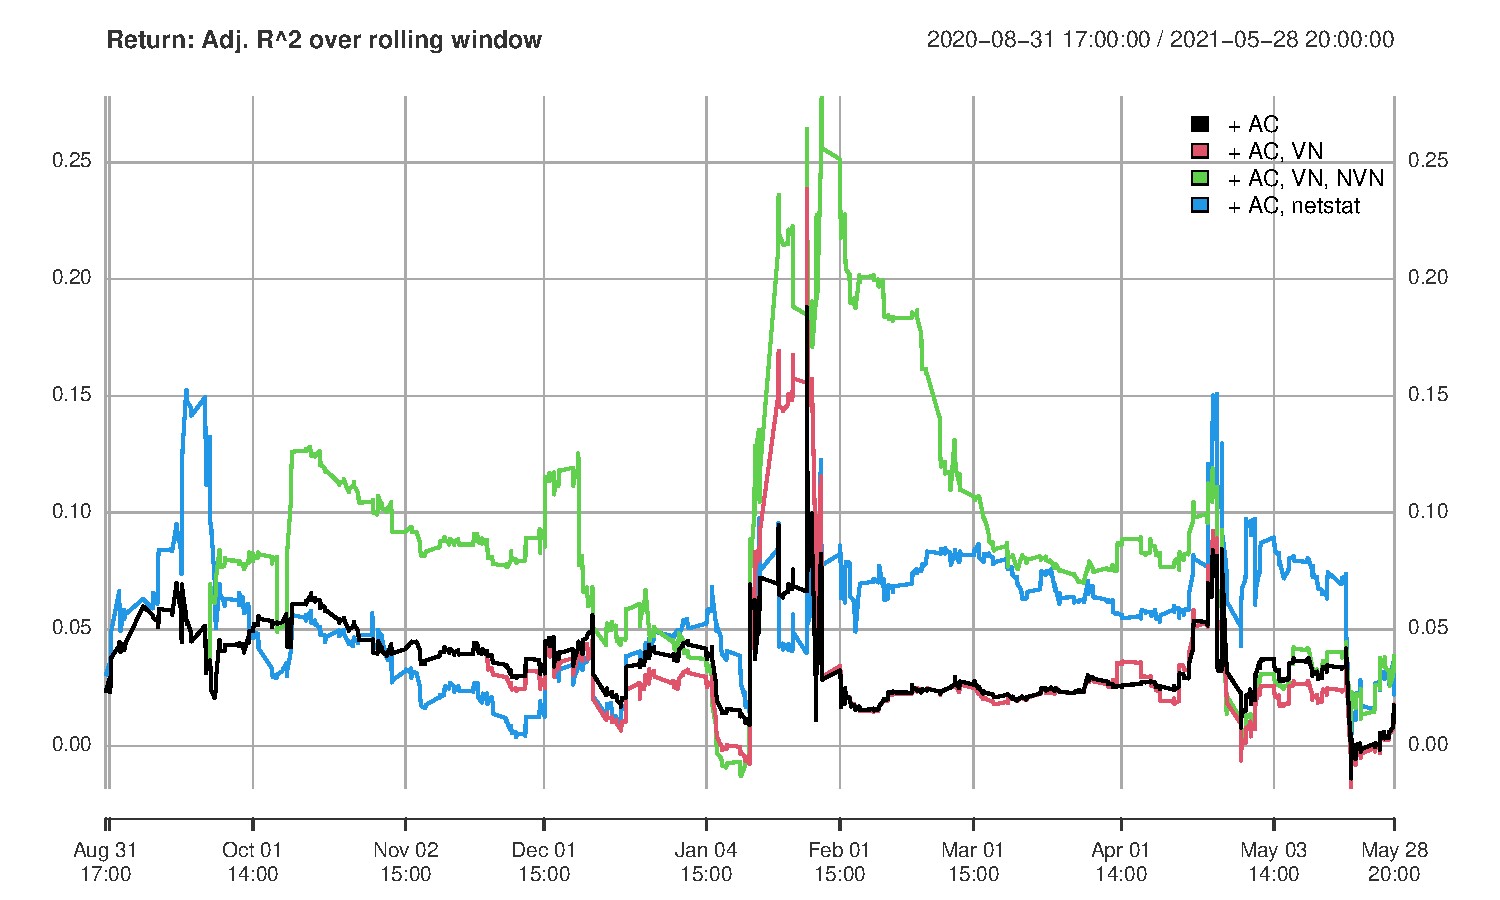
\includegraphics[scale = 0.5]{adjR2_return_rolling.pdf}
\end{figure}


%\input{Volumemodels1_t.tex}

%Turning towards integrated and jump volatility, an interesting pattern emerges, compare Figures \ref{fig:rolling_iv} and \ref{fig:rolling_jv}. Note that the models are similar to the return one, but that the jump volatility model does not contain past jumps as explainable variable as jumps are independent and random by definition. For integrated variance, we observe that the change points of VN and ANVN excel in explaining its dynamic with the onset of the market frenzy. After the frenzy, the explainability from the changes in users behaviour remain high and excel in explaining its dynamics compared to all other model specifications. Even values of up to $0.7$ in adjusted $R^2$ are observed following the market frenzy whereas the next best model only reaches $0.4$. This infers that the role the social network played in the market frenzy, in particular individual users change in behaviour, caused a longer running change in the drivers of integrated variance. 

%For jump volatility, Figure \ref{fig:rolling_jv}, we observe a remarkably high explainability from the users' change in behaviour. Already months before the actual market frenzy, the users change in behaviour explained for a while $80\%$ of the jump dynamics (adj. $R^2$), before dropping to a range of $20-40\%$. Note that leaving out the changepoints as explainable variables from the model resulted in tremendously lower explainability of the jump dynamics, consistently way below the VN and ANVN changepoint model. Note that no model was able to explain the jump dynamics during December, but with the onset of the market frenzy, again the changes in users behaviour strongly improved the explainability of the occurrence of jumps in volatility. Towards the mid of the year, months after the market frenzy took place, explainability of users change in behaviour increased again and outperformed other specifications. 
%For trading volume, Figure \ref{fig:rolling_tv}, we observe a mixed picture. Overall the adjusted $R^2$ is low for all model specifications, but the change in users behaviour hardly ever explains the trading volume dynamics better than other variables. Only during the period of the direct aftermath of the market frenzy, the changes in users' behaviour improve the trading volume explainability. 

In summary, these results show that the changes in users behaviour have a strong and long lasting effect on the return dynamics. In particular, changes in ANVN-users behaviour excel in doing so, VN-users play a lesser role in explaining the return dynamics. This implies that not only highly influential users, despite inciting communication in the network, had an effect on the market. Their impact is comparably less pronounced than the changes in behaviour emerging from the masses of users on the social network. 

%We also investigate if the detection of the changepoints and their explainability for the dynamics of the integrated variance could be proxied by the network measures mean distance, mean degree and number of active nodes. These measures proxy network activity and importance of nodes. However, including them instead of the $VN$ and $NVN$ changepoints, yields a tremendously lower $R^2$ of $0.255$ compared to $0.392$ when $VN$ and $NVN$ are included but the network control statistics are not. 
%
%As we established, the changepoints have a strong and significant impact on the integrated variance. On the jump component, $JV$, which is by its nature a short-lived part of the variance, the change in behaviour of users has less of an impact, compare Table \ref{Jmodels1_t}. The $R^2$ increases strongly with the exponential weighting specifications for the changes behaviour, (\ref{eq:spec2}), however the impact is not as strong as for the network statistics. Given this is the jump component of the variance, this infers that the change in users behaviour is not strongly related to the immediate excesses in the GME variance. However it is strongly related to the integrated part of the variance, hence the regular variance. 
%
%We further investigate if not only the variance of GME is explained by the behaviour of users on WSB, but also if the return of GME is determined by it. We observe a persistent increase in terms of $R^2$ and also adjusted $R^2$ when adding network activity and the vital nodes changepoints, VN, to the model comprised of the hourly lagged return of GME, compare Table \textcolor{red}{TABLE HAS NO LABEL YET}. The largest increase takes place when the changepoints of the Non-Vital Nodes, ANVN, is being added to the model. We observe a $R^2$ and adjusted $R^2$ of 0.132 and 0.115 respectively. We observe that all ANVN variables, the contemporaneous and lagged ones, are significant and in combination with the drastically increasing model fit, we conclude that the changepoints of the Non-Vital Nodes has high explainability for the GME return evolution. The model containing only the network statistics does not reach achieve an equally high $R^2$, consequently the VN and ANVN indeed explain the return movements of GME better than established network statistics. Adding said network statistics to the model containing also the VN and ANVN, achieves an even higher $R^2$ and adjusted $R^2$, which suggests that the VN and ANVN explain part of the return movements which are not captured by the network statistics, network activity and also not by the past return movements. 
%
%Likewise we investigate if the dynamics of the trading volume (TV) of GME is explained by the changepoints of the Vital Nodes (VN) and Non-Vital Nodes (NVN). We observe that the variables embedded in model (\ref{eq:vol}) explain parts of the dynamics of the trading volume. The $R^2$ and adjusted $R^2$ reach the best values for the model containing the past trading volume, network activity and VN. Note that the VN parameter is significant whereas none of the AC parameters is significant. We observe that adding the ANVN and network statistics causes a decrease in the adjusted $R^2$, conseqeuntly including them only marginally increases the explainability of the system. As in the previous examinations, we conclude that the changepoints of the vital nodes, VN, explain the dynamics of the trading volume. 

%The baseline model we compare against contains the parameters $r_{t-1}$ and $AC_{t}$ for the contemporaneous model and $r_{t-1}$ and $AC_{t-1}$ for the time lagged model. This specification follows the markov property that past returns predict future ones and that the activity of a network impacts related stock returns. We observe that for the contemporaneous model, the parameter $AC_{t}$ is significant and the $R^2$ is $0.016$. When adding $cp_{vn;t}$ and $cp_{nvn;t}$ to the model, the network variable parameter becomes insignificant while the $R^2$ increases as well as the adjusted $R^2$, Table \ref{table_return_contem}. Simultaneously $cp_{vn;t}$ is significant which suggests that the actual reason for the observation that the network activity impacts the return of GME, the actual reason for this was the change in behaviour of vital nodes on the Wallstreetbets network. Given that alternative measures for a networks state such as mean degree, distance and active nodes exist, we add these variables to the model which increases the $R^2$. Notably the vital nodel changepoint variable remains significant. 

%Considering that changes in ones behaviour are not an isolated event but rather an event with a potentially lasting effect for a while, we analyse if $cp_{vn,ews;t}$ and $cp_{nvn,ews;t}$ impacts the return. We set $\lambda = 0.8$. Again, the changepoints of the vital nodes are significant and also the ones for the non-vital nodes become significant. Notably the $R^2$ increases as does the adjusted $R^2$. 

%After having established that the contemporaneous effect of the changepoints impacts the market return of GME, we investigate the time lagged effect, Table \ref{table_return_timelagged}. The results remain similar which shows that also past changepoints of vital and non-vital nodes impacts the returns of GME. Notably the $R^2$ decreases compared to the contemporaneous model however the significance of the parameters remains. 

%In a similar setup as for the return, we are analysing if the Wallstreetbets network and the changepoints of the nodes impact the realized volatility of GME, compare Tables \ref{table_rv_contem} nad \ref{table_rv_timelagged}. Again the baseline model is the time lagged realized volatility and contemporaneous activity with both parameters being significant and a $R^2$ of $0.13$. After adding the parameters $cp_{vn;t}$ and $cp_{nvn;t}$, we observe the latter to be significant and an increase in $R^2$. The parameter $AC_{t}$ becomes insignificant however the parameter is strongly correlated with $cp_{nvn;t}$. When adding the additional network variables the R$R^2$ further increases. Replacing the parameters $cp_{vn;t}$ and $cp_{nvn;t}$ with $cp_{vn,ews;t}$ and $cp_{nvn,ews;t}$ ($\lambda = 0.8$), we observe a strong increase in $R^2$ to $0.21$ and the parameter $cp_{vn,ews;t}$ becomes significant. This result provides further evidence that the change in behaviour of the vital nodes in the network impacts the GME stock. 

%When considering the time lagged model for the realized volatility, we observe similar results for the parameters in terms of significance and the $R^2$ is much higher than for the contemporaneous one, reaching up to $0.25$. This result shows the importance of the changepoints of the vital nodes for the performance of the GME stock and hence the traders of the stock.
%\textit{here results about the impact of users posting behaviour and changes in their behaviour on the GME stock price}



%\begin{figure}
%	\caption{Adj. $R^2$ for integrated variance models with rolling window over 3 months with step width 1 hour.}
%	\label{fig:rolling_iv}
%	\centering
%	\includegraphics[scale = 0.5]{adjR2_iv_rolling.pdf}
%\end{figure}
%
%\begin{figure}
%	\caption{Adj. $R^2$ for jump volatility models with rolling window over 3 months with step width 1 hour.}
%	\label{fig:rolling_jv}
%	\centering
%	\includegraphics[scale = 0.5]{adjR2_jv_rolling.pdf}
%\end{figure}
%
%\begin{figure}
%	\caption{Adj. $R^2$ for trading volume models with rolling window over 3 months with step width 1 hour.}
%	\label{fig:rolling_tv}
%	\centering
%	\includegraphics[scale = 0.5]{adjR2_tv_rolling.pdf}
%\end{figure}


\subsubsection{5-minute analysis: The network during the market frenzy}
%\label{fin_analysis_frenzy}
\label{sec:5minby5min}
%For a detailed look at the microstructure of the network around the frenzy, we construct similar networks as before on a 5 minute frequency. Again, we apply our ISBM methodology. %the models from Equations \ref{eq:infl_model} and \ref{eq:mod_fol} to the VNs and ANVNs. We combine the models with the change point detection method described in Section \ref{sec:cps} and link them to the market thourgh . 
%The results are inline with the results we find for the full year model based on hour-by-hour data (as presented in Section \ref{sec:hourbyhour}), hence we  refer the interested reader to the online Appendix for a detailed analysis.

%(11 Jan 2021 until 13 Feb 2021) in Section \ref{sec:5minby5min}. Note that the price peaked on 26 Jan, which marks the centre of this window.

A particular period of interest for GME is the time spanning the market frenzy. During this time we also observed that a lot more activity took place on WSB, consequently we zoom in on the market frenzy. We construct similar networks as before on a 5 minute frequency for the period 11 Jan 2021 until 13 Feb 2021. Note that the price peaked on 26 January, which marks the centre of this window. We apply the ISMB modelling approach to this data using market variables constructed from minute-by-minute data. %the market movements and their relations to the user behaviour on WSB. 
The results remain largely similar to the ones from the hour-by-hour analysis, with the notable exception that the effect of the change points of the VN and ANVN is less pronounced during the market frenzy than during the entire time period. We attribute this to the fact that during the frenzy, the market was a lot more volatile than before and actions taking place outside of WSB played a notable role for the market movements, such as a ban of Robinhood, the main trading app for WSB investors, on buying GME. Since the results support the findings made so far, we refer the interested reader to the Appendix \ref{appendix} for a detailed analysis.



\subsection{Reverse causality}
\label{reverse_causality}

Since we found that the change points of the VN and ANVN explain market movements, we also investigate if the opposite holds true, i.e. if the change points of the VN and ANVN result from the returns of GME. \str{We regress the hourly change points of the VN and ANVN with 7 Lags, the past 7 hourly AC variables, events associated with the WSB frenzy as count variable, and the past 7 hourly returns, onto the present VN and ANVN variable realisation. The events are obtained from \cite{GMETimeline}. If more than one event occur on a given day, we record the count of events for the day. The count of events is regressed upon the count of change points of the VN and ANVN on the same day. With this we control for a higher/lower count being associated with the occurrence of external events on that day. To determine if the relationship is different during the build-up to the frenzy, the frenzy period, and its aftermath, we take the splits used for the 5 minute analysis as start and end of the frenzy period. Left are the observations used before 2021-01-11, middle between 2021-01-11 and 2021-02-13, and after 2021-02-14. The results are displayed in Tables \ref{NVN_reg_robust} and \ref{VN_reg_robust}. We observe that none of the parameters associated with return and events is significant. This infers that the change points of the VN and ANVN do not result from the returns on the markets, instead the cause for them originates in the network. Hence we follow that reverse causality is not present and the change points are not a result of changes in market returns or the occurrence of external events.
}

\str{We investigate if the variables we constructed from the change points of the VN and ANVN are uniquely associated with GME. Since our analysis showed that the change points do not or only weakly effect the trading and option trading volume, we focus this robustness test onto the return, IV, and JV, for which we observed notable effects. We obtain the hourly price series of the stocks 3M (MMM), Cisco (CSCO), and General Electric (GE), which represent different sectors of the U.S. economy and are reasonably unrelated to the events surrounding the GME market frenzy. From the price series, we obtain the hourly log return, IV, and JV, in the same manner as for GME. We derive the baseline model, (1), which only contains the lagged variable itself with 7 Lags. For JV, no model is computed as past jump volatility does not predict future jump volatility by construction, same as for the main analysis. Model (4) contains additionally the variables associated with AC, VN, and ANVN with 7 lags, same as for the main analysis. Model (6) contains additionally the network statistics. With the naming convention (1), (4), (6), we follow the naming of the main analysis. We report the adj. $R^2$ for each model for return, IV, JV of the three stocks, see Table \ref{table_MMM_CSCO_GE}. We see that adding the variables for AC, network statistics, and change points for VN and ANVN from GME to the equations, results in almost no adj. $R^2$ improvement, even negative values frequently occur. The increases observed for IV are minor and not comparable with the improvements we observed for GME. This shows that the effects from the change points of the VN and ANVN are specific to GME. }



% Table created by stargazer v.5.2.3 by Marek Hlavac, Social Policy Institute. E-mail: marek.hlavac at gmail.com
% Date and time: Mon, Oct 19, 2026 - 17:03:18
\begin{table}[!htbp] \centering 
  \caption{Regression to determine if the returns lead to the changepoints. We regress 
onto the NVN variables their past 7 lagged variables, past 7 AC variables, events associated with the WSB frenzy as count variable, and 
the past 7 returns. To determine if the relationship is different during the build-up to the frenzy, the frenzy period, and its aftermath, we 
take the splits used for the 5 minute analysis as start and end of the frenzy period. Left are the observations used before 2021-01-11, middle between 2021-01-11 and 2021-02-13, and after 
2021-02-14. We observe that the returns over 7 lags do not significantly impact the change point variables, 
hence the cause for the changepoints occurrence originates in the network.} 
  \label{NVN_reg_robust} 
\scriptsize 
\begin{tabular}{@{\extracolsep{5pt}}lccc} 
\\[-1.8ex]\hline 
\hline \\[-1.8ex] 
 & \multicolumn{3}{c}{\textit{Dependent variable:}} \\ 
\cline{2-4} 
\\[-1.8ex] & \multicolumn{3}{c}{NVN} \\ 
\\[-1.8ex] & (1) & (2) & (3)\\ 
\hline \\[-1.8ex] 
 NVN1 & 0.193$^{***}$ & 0.621$^{***}$ & 0.688$^{***}$ \\ 
  & (0.039) & (0.101) & (0.042) \\ 
  & & & \\ 
 NVN2 & 0.013 & $-$0.029 & 0.160$^{***}$ \\ 
  & (0.039) & (0.105) & (0.047) \\ 
  & & & \\ 
 NVN3 & 0.104$^{***}$ & 0.095 & 0.008 \\ 
  & (0.038) & (0.075) & (0.036) \\ 
  & & & \\ 
 NVN4 & 0.006 & $-$0.024 & $-$0.085$^{**}$ \\ 
  & (0.035) & (0.077) & (0.033) \\ 
  & & & \\ 
 NVN5 & $-$0.108$^{***}$ & $-$0.072 & 0.006 \\ 
  & (0.029) & (0.071) & (0.032) \\ 
  & & & \\ 
 NVN6 & $-$0.009 & 0.141$^{**}$ & 0.086$^{***}$ \\ 
  & (0.026) & (0.067) & (0.030) \\ 
  & & & \\ 
 NVN7 & 0.024 & $-$0.049 & 0.011 \\ 
  & (0.025) & (0.060) & (0.028) \\ 
  & & & \\ 
 AC & $-$0.024 & 0.085 & 0.063 \\ 
  & (0.016) & (0.138) & (0.050) \\ 
  & & & \\ 
 AC1 & 0.029 & $-$0.127 & $-$0.074 \\ 
  & (0.019) & (0.153) & (0.067) \\ 
  & & & \\ 
 AC2 & 0.004 & $-$0.077 & 0.059 \\ 
  & (0.020) & (0.169) & (0.071) \\ 
  & & & \\ 
 AC3 & 0.006 & 0.328 & $-$0.065 \\ 
  & (0.021) & (0.286) & (0.073) \\ 
  & & & \\ 
 AC4 & 0.013 & $-$0.194 & 0.001 \\ 
  & (0.021) & (0.245) & (0.071) \\ 
  & & & \\ 
 AC5 & $-$0.020 & 0.174 & 0.00005 \\ 
  & (0.019) & (0.207) & (0.069) \\ 
  & & & \\ 
 AC6 & $-$0.003 & $-$0.238 & $-$0.035 \\ 
  & (0.017) & (0.213) & (0.068) \\ 
  & & & \\ 
 AC7 & 0.031$^{**}$ & 0.126 & 0.159$^{***}$ \\ 
  & (0.013) & (0.157) & (0.048) \\ 
  & & & \\ 
 ret1 & 1.781$^{*}$ & 0.805 & $-$0.038 \\ 
  & (1.009) & (1.831) & (1.548) \\ 
  & & & \\ 
 ret2 & 0.900 & $-$1.988 & $-$2.084 \\ 
  & (1.026) & (1.729) & (1.540) \\ 
  & & & \\ 
 ret3 & 0.903 & 0.870 & 1.574 \\ 
  & (1.020) & (1.704) & (1.539) \\ 
  & & & \\ 
 ret4 & 1.187 & 1.334 & 0.882 \\ 
  & (1.019) & (1.695) & (1.550) \\ 
  & & & \\ 
 ret5 & $-$1.186 & $-$1.313 & 0.854 \\ 
  & (1.015) & (1.768) & (1.530) \\ 
  & & & \\ 
 ret6 & 0.563 & 2.611 & 0.799 \\ 
  & (1.007) & (1.805) & (1.498) \\ 
  & & & \\ 
 ret7 & $-$1.300 & 1.206 & $-$0.662 \\ 
  & (1.006) & (1.690) & (1.500) \\ 
  & & & \\ 
 event & 0.034$^{**}$ & $-$0.001 & 0.053 \\ 
  & (0.016) & (0.164) & (0.066) \\ 
  & & & \\ 
 Constant & $-$0.045$^{***}$ & $-$0.162 & $-$0.483$^{***}$ \\ 
  & (0.010) & (0.359) & (0.118) \\ 
  & & & \\ 
\hline \\[-1.8ex] 
Observations & 975 & 160 & 505 \\ 
R$^{2}$ & 0.167 & 0.445 & 0.935 \\ 
\hline 
\hline \\[-1.8ex] 
\textit{Note:}  & \multicolumn{3}{r}{$^{*}$p$<$0.1; $^{**}$p$<$0.05; $^{***}$p$<$0.01} \\ 
\end{tabular} 
\end{table} 


% Table created by stargazer v.5.2.3 by Marek Hlavac, Social Policy Institute. E-mail: marek.hlavac at gmail.com
% Date and time: Mon, Oct 19, 2026 - 17:03:20
\begin{table}[!htbp] \centering 
  \caption{Regression to determine if the returns lead to the changepoints. We regress 
onto the VN variables their past 7 lagged variables, past 7 AC variables, events associated with the WSB frenzy as count variable, and 
the past 7 returns. To determine if the relationship is different during the build-up to the frenzy, the frenzy period, and its aftermath, we 
take the splits used for the 5 minute analysis as start and end of the frenzy period. Left are the observations used before 2021-01-11, middle between 2021-01-11 and 2021-02-13, and after 
2021-02-14. We observe that the returns over 7 lags do not significantly impact the change point variables, 
hence the cause for the changepoints occurrence originates in the network.} 
  \label{VN_reg_robust} 
\scriptsize 
\begin{tabular}{@{\extracolsep{5pt}}lccc} 
\\[-1.8ex]\hline 
\hline \\[-1.8ex] 
 & \multicolumn{3}{c}{\textit{Dependent variable:}} \\ 
\cline{2-4} 
\\[-1.8ex] & \multicolumn{3}{c}{VN} \\ 
\\[-1.8ex] & (1) & (2) & (3)\\ 
\hline \\[-1.8ex] 
 NVN1 & 0.012 & $-$0.013 & 0.005 \\ 
  & (0.008) & (0.012) & (0.007) \\ 
  & & & \\ 
 NVN2 & $-$0.013 & 0.008 & $-$0.0005 \\ 
  & (0.008) & (0.013) & (0.008) \\ 
  & & & \\ 
 NVN3 & 0.028$^{***}$ & $-$0.005 & 0.0002 \\ 
  & (0.008) & (0.009) & (0.006) \\ 
  & & & \\ 
 NVN4 & 0.017$^{**}$ & 0.0003 & $-$0.002 \\ 
  & (0.007) & (0.010) & (0.006) \\ 
  & & & \\ 
 NVN5 & $-$0.019$^{***}$ & $-$0.0004 & $-$0.003 \\ 
  & (0.006) & (0.009) & (0.006) \\ 
  & & & \\ 
 NVN6 & $-$0.004 & $-$0.006 & $-$0.002 \\ 
  & (0.005) & (0.008) & (0.005) \\ 
  & & & \\ 
 NVN7 & 0.009$^{*}$ & 0.002 & 0.001 \\ 
  & (0.005) & (0.007) & (0.005) \\ 
  & & & \\ 
 AC & $-$0.001 & 0.007 & $-$0.002 \\ 
  & (0.003) & (0.017) & (0.009) \\ 
  & & & \\ 
 AC1 & 0.001 & 0.002 & 0.010 \\ 
  & (0.004) & (0.019) & (0.011) \\ 
  & & & \\ 
 AC2 & 0.001 & 0.001 & $-$0.002 \\ 
  & (0.004) & (0.021) & (0.012) \\ 
  & & & \\ 
 AC3 & $-$0.001 & $-$0.003 & 0.009 \\ 
  & (0.004) & (0.035) & (0.012) \\ 
  & & & \\ 
 AC4 & 0.002 & 0.030 & $-$0.011 \\ 
  & (0.004) & (0.030) & (0.012) \\ 
  & & & \\ 
 AC5 & $-$0.002 & 0.00003 & 0.006 \\ 
  & (0.004) & (0.026) & (0.012) \\ 
  & & & \\ 
 AC6 & 0.002 & $-$0.014 & $-$0.006 \\ 
  & (0.004) & (0.026) & (0.012) \\ 
  & & & \\ 
 AC7 & $-$0.001 & $-$0.011 & 0.001 \\ 
  & (0.003) & (0.019) & (0.008) \\ 
  & & & \\ 
 ret1 & $-$0.076 & 0.031 & $-$0.453$^{*}$ \\ 
  & (0.206) & (0.226) & (0.263) \\ 
  & & & \\ 
 ret2 & $-$0.055 & 0.179 & $-$0.091 \\ 
  & (0.210) & (0.213) & (0.262) \\ 
  & & & \\ 
 ret3 & $-$0.125 & 0.018 & $-$0.289 \\ 
  & (0.208) & (0.210) & (0.262) \\ 
  & & & \\ 
 ret4 & $-$0.082 & 0.196 & 0.101 \\ 
  & (0.208) & (0.209) & (0.264) \\ 
  & & & \\ 
 ret5 & $-$0.122 & $-$0.023 & $-$0.158 \\ 
  & (0.207) & (0.218) & (0.260) \\ 
  & & & \\ 
 ret6 & $-$0.233 & 0.301 & 0.141 \\ 
  & (0.206) & (0.223) & (0.255) \\ 
  & & & \\ 
 ret7 & 0.055 & $-$0.004 & $-$0.159 \\ 
  & (0.206) & (0.209) & (0.255) \\ 
  & & & \\ 
 event & $-$0.005 & $-$0.031 & $-$0.004 \\ 
  & (0.003) & (0.020) & (0.011) \\ 
  & & & \\ 
 Constant & $-$0.001 & $-$0.027 & $-$0.006 \\ 
  & (0.002) & (0.044) & (0.020) \\ 
  & & & \\ 
\hline \\[-1.8ex] 
Observations & 975 & 160 & 505 \\ 
R$^{2}$ & 0.039 & 0.076 & 0.021 \\ 
\hline 
\hline \\[-1.8ex] 
\textit{Note:}  & \multicolumn{3}{r}{$^{*}$p$<$0.1; $^{**}$p$<$0.05; $^{***}$p$<$0.01} \\ 
\end{tabular} 
\end{table} 


% latex table generated in R 4.5.0 by xtable 1.8-4 package
% Tue Oct 20 17:33:48 2026
\begin{table}[ht]
\centering
\caption{This table shows the adj. $R^2$ from deriving model specifications (1), (4), and (6) with the log return, IV, and JV of the three stocks 
                    MMM, CSCO, and GE respectively, instead of GME. The baseline model, (1), contains only the lagged variable itself with 7 Lags. For JV, no model is computed as past jump volatility does not predict future jump volatility by construction. We see that adding the variables for 
                    AC, network statistics, and change points for VN and ANVN from GME to the equations, results in almost no adj. $R^2$ improvement, even negative values frequently occur. 
                    The increases observed for IV are minor and not comparable with the improvements we observed for GME. This shows that the effects from the change points of the VN and ANVN
                    are specific to GME.} 
\label{table_MMM_CSCO_GE}
\begingroup\scriptsize
\begin{tabular}{l|rrr|rrr|rrr}
   \hline \hline
 &   & MMM &   &   & CSCO &   &   & GE &   \\ 
   & (1) & (4) & (6) & (1) & (4) & (6) & (1) & (4) & (6) \\  \hline
  Return & 0.0013 & 0.0017 & 0.0039 & 0.0006 & -0.0057 & -0.0065 & -0.0013 & 0.0003 & -0.0019 \\ 
  IV & 0.1324 & 0.1405 & 0.1509 & 0.2244 & 0.2399 & 0.2438 & 0.0726 & 0.086 & 0.0985 \\ 
  JV & 0 & -0.005 & -0.004 & 0 & -0.0116 & -0.0242 & 0 & -0.0036 & 0.0077 \\ 
    \hline Lagged variable (for JV No) & Yes & Yes & Yes & Yes & Yes & Yes & Yes & Yes & Yes \\ 
    Vital nodes & No & Yes & Yes & No & Yes & Yes & No & Yes & Yes \\ 
    Non-vital nodes & No & Yes & Yes & No & Yes & Yes & No & Yes & Yes \\ 
    Network activity & No & Yes & Yes & No & Yes & Yes & No & Yes & Yes \\ 
    Network statistics & No & No & Yes & No & No & Yes & No & No & Yes \\ \hline
\hline
\end{tabular}
\endgroup
\end{table}


\subsection{Financial and economic implications}
\label{econ_implications}
Our results show that there exists a link between individual users behaviour upon social networks and market behaviour. This provides not only empirical justification for the theoretical model by \textcite{Pedersen2022}, but also shows the necessity to quantify individual users behaviour on social networks instead of aggregating over all users, as commonly done in many research studies. This necessity derives from the demonstrated relationship between individual users change in behaviour and market movements, which cannot be proxied for with aggregated network statistics. 

The VNs take up a central role in this relationship, even though their own change in behaviour explains less market movements than the ones from ANVNs. 
VNs change in behaviour results after 6 hours in a significant effect upon market dynamics. This makes sense since a post by a single influential person first needs to reach a credible number of investors to lead to market reactions. While it is extremely challenging to detect change points in large social networks quickly \citep{Yu2022monitoring,zwetsloot2025online}, this suggests that influential users change in behaviour could act as an early warning sign for meme stock market reactions, if identified early enough. We also find that several influential users exhibit a change in behaviour 1-2 months before the market frenzy. %This paves the way towards an early warning signal for meme stock market frenzies. 
Lesser influential users (ANVNs) change in behaviour, if occurring in bulk, ripples instantly and with a various hours lasting effect into the financial markets. Their change in behaviour explains the largest portion of market dynamics, even when controlling for network activity. This finding paves the way towards the construction of variables for stock market movements based on social network users change in behaviour. 

These findings emphasise the need to detect and monitor (change in behavior of) highly influential users, but it also shows the need to monitor their followership closely as it is their change in behaviour which explains an even larger part of market movements. 




%\subsubsection{Modeling by trading hours}
%\label{fin_analysis_tradinghours}
%We investigate if the results of our study hold up when we focus the analysis upon the trading hours of NYSE and compute one model per trading hour. By this, we investigate if seasonality of trading is impacting our results. As there are 7 trading hours, this leads to 7 models for each of the time series to be analysed, namely return, integrated volatility, jump volatility and trading volume. The results indicate that the change in posting behaviour of the VNs and ANVNs plays an even stronger role when focusing upon the individual trading hours. Across the hours and data series, the $R^2$ and adj. $R^2$ are much higher. For the return series, Table \ref{table_hourly_RET}, we observe that for all hours but the first and last one, a higher proportion of the variability is explained by the change points of VN and ANVN compared to the network statistics. In all cases, considering the change points and network statistics improves the $R^2$ and adj. $R^2$ the most. Notably the models strongly outperform a standard autoregressive model. For hour 5, the AR model only yields 0.1 adj $R^2$ but the model considering AC and the change points of VN and ANVN yields 0.48 adj $R^2$. Since the results support the findings made so far, we refer for the further analysis of the return, integrated variance, jump volatility and trading volume to Appendix \ref{app:app_modelbyhour}. 

%\subsection{Robustness of VN definition}
%\label{fin_analysis_VNdefinition}
%In Definition \ref{def:infl} we postulate a definition for vital nodes as \emph{those nodes in the network that submit posts in at least 10\% of the weeks and receive the highest 10\% median comments on their posts.} This is a relaxed definition as it only requires posting activity in 5 weeks. To validate if a stricter definition of a vital node would impact the results of the study, we investigate the robustness of the results subject to the definition by rerunning the analysis while adapting this definition. 
%We amend the VN definition by the posting frequency and amount of comments. We redefine a VN as communicating in at least 15\% and 20\% of the weeks (ie more frequently). In addition, the 10\% median comments is also validated by requiring the highest 5\% median comments (making it stricter). Regardless of the definition for the vital nodes, we observe that the identified change points strongly improve the modelling of the return, integrated variance, jump volatility and trading volume. Notably, we observe that for several instances, the base setting of this study, `10-10', leads to a lower $R^2$ and adj. $R^2$ than other settings. This result let us to using `10-10' as the base setting for this study. Hence we conclude that the results of the study are robust towards the VN definition and that the chosen definition is a conservative choice. For a detailed analysis, we refer the interested reader to Appendix \ref{app:vnrobust}. 

%\textit{here the results of the minute-by-minute modelling of the users behaviour during the market frenzy in January 2021}







\section{Discussion and Conclusion}
\label{sec:conclusion}
%conclusion
%\hl{I have expanded the conclusion to fit IRSs structure. This should be rewritten once the paper is in a more final form}

%\subsection{Summary of work}
In this study, we investigate the drivers and changes in users' posting probability on social networks via a sparse network model and change point detection modelling approach. For the study we collected 3.8 million posts from 502,650 users from WallStreetBets, a subreddit. We examine the impact of individual user behaviour on the Reddit forum Wallstreetbets upon markets. Thereby we provide empirical validation for the theoretical model developed by \citet{Pedersen2022} as well as extending prior research that focuses on aggregated network measures only. 

The DeGroot type model of \citet{Pedersen2022} is a theoretical framework for understanding (meme) stock prices discussed and traded by users of social networks. It being a DeGroot model implies that users of the network change their opinions towards a stock as a result of information they receive from the network, which translates then into price changes. 
Our results demonstrate that changes in users' behaviour significantly explained returns, integrated volatility, and jump volatility, even when controlling for network activity and established metrics measuring influential user impact. We also show that the change in behaviour is not explained by market dynamics, instead it is rooted in the activity on the social network. Including changes in behaviour of users on Reddit into models to explain the market movements, leads to improvements in the modeling fit.
%, leads to an increase in adjusted $R^2$ of $630\%$ for return explainability. %up to $0.45$ for return and $0.8$ for jump explainability, vastly outperforming the competing models. 

Studies often focus upon influential users in networks, but we show that changes in behaviour of less important users explain a larger part of returns, integrated variance and jump volatility than important users do. Influential users change in behaviour results after 6 hours in a significant effect upon market dynamics. This makes sense since a post by a single influential person first needs to reach a credible number of investors before eliciting market reactions. Lesser influential users change in behaviour, if occurring in bulk, ripples instantly and with a various hours lasting effect into the financial markets. Their change in behaviour explains the largest portion of market dynamics, even when controlling for network activity. This finding paves the way towards the construction of variables for stock market movements based on social network users change in behaviour. 

%It has been shown that network activity such as aggregated number of posts at a given time is an important factor in modeling network influence on markets \parencite{Audrino2020, Gan2020, Jiao2020}. While controlling for these and other effects, we study the relationship between the changepoints in the behaviour of individual vital and non-vital users and the market behaviour of GME. We analyse the effect of users change in behaviour on the integrated and jump volatility which we derive from hourly and 5 minute realized volatility, hourly and 5 minute trading volume as well as the corresponding returns. 
%The results show that the change in behaviour of vital and non-vital nodes strongly improves the predictability of said metrics. The adj. $R^2$ from a model without vs. with variables representing behavioural change of individual users, improves by $150\%$. During the market frenzy, these variables contribute towards reaching $0.45$ adj. $R^2$. Likewise for integrated variance, the changepoints of the vital/non-vital nodes excel in explaining market dynamics with the onset of the market frenzy. For jump volatility, even $0.8$ adj. $R^2$ is reached. Even better market predictability is reached when considering to build the models as by trading hour. Given we observe that the developed network model outperforms established metrics for measuring influential user impact, we conclude that the proposed methodology provides a viable framework to investigate a nodes behaviour over time. 

%It is remarkable, that classical network measures such as network activity and network statistics were not able to explain the market movements that well. The explainability of the return dynamics from the changes of users behaviour remained high also after the frenzy, outperforming all other models. This shows that the social network had a longer lasting effect on the markets, going beyond the main market frenzy. 

%\subsection{Theoretical Implications}
%Using our method we address an important gap in the existing literature on the relationship between social networks and stock markets. Our approach focuses on the network micro structure and links individual users' behaviour to stock market behaviour. We show that including this individual change in behaviour results in a larger $R^2$ compared to just aggregated network measures, showing that not only vital nodes in the network but all nodes are important to incorporate. 

Our modelling approaches applicability extends well beyond the scope of the study. With the ever growing number of meme stocks, our method can be used to analyse the impact users on social media have upon market prices. 
While it is extremely challenging to detect change points quickly, our findings suggest that influential users change in behaviour could act as an early warning signal for meme stock market reactions, if identified early enough. We also find that several influential users exhibit a change in behaviour 1-2 months before the market frenzy. %This paves the way towards an early warning signal for meme stock market frenzies. 
Further, our method is applicable to meme coins, which have similar origins as meme stocks. Due to the ease of creating new cryptocurrencies, the market of meme coins is persistently growing and our model provides a method to determine the effect social network users have upon meme coins. 

%\subsection{Practical Contributions}
%Our paper has important managerial implications. First, our findings provide implications for Reddit and other online platforms. Understanding the relationship between online communications on social networks and stock markets helps platforms understand the importance of their role in the economy. Second, meme stocks are having a real impact on funds’ values; however, this influence is extremely unpredictable and volatile. Thus, for fund and portfolio management, a thorough understanding of network evolution and the underlying driving factors is crucial. Our model provides important insights on the relationship between social network discussions and stock prices. Third, a better understanding of the relationship between online social networks and financial markets is crucial for regulators. For these stakeholders, we offer a framework to study the nature of the effect of social networks upon stock markets behaviour.  %within which this phenomenon can be studied. Our research provides guidance to regulators to understand the dynamics on networks and the relationship with the stock market. It shows that we should monitor both the leaders as well as the `crowd' as they can have profound influence upon stock markets. We also 

%\subsection{Limitations and Future Research Opportunities}
This study sets the stage for a number of potential future research opportunities. We show in this study that individual users change in behaviour explains market movements. The GME market frenzy led to the emergence of various meme stocks, with some of them emerging shortly after the market frenzy, such as AMC and BB. A potential future research opportunity would be to study the spillover of the GME frenzy into these assets market frenzies and vice versa. In this study, we distinguish between the relationship of change in behaviour of vital and admissible non-vital users with market movements and show that the studies' results are robust towards different definitions for vital users. An interesting research question is the relationship between individual vital nodes and the admissible non-vital nodes associated with them, which would shed light onto the incremental role single users played in the market frenzy. %network models require variables and structures which suit the network architecture of the social network under investigation. Our study provides a model for the Reddit social network and a different social network would require an extension of the model to its specific architecture. Further, during the study we tested a number of algorithms to detect vital nodes in the network and found them to work not adequately, leading us towards designing a method for vital node identification. Accordingly, future research could design algorithms to identify vital nodes in a dynamic network. 
%As an initial attempt to model and analyze the relationship between individual social network user behavior and stock market analysis this study is prone to several limitations that offer opportunities for future research. First, the current paper focuses on the link structure of a network, an important and interesting extension would be to include the content of posts as well as nodal characteristics to this analysis as \citet{han2020importance} show that the interaction between those two is an important factor determining virality of content in social networks. Second it is challenging to implement our current modeling prospectively due to the manner in which we search change points over a window. Future research should focus on finding changepoint prospectively. Existing appraoches for prospective change detection in networks, such as \cite{zwetsloot2025online}, all focus on aggregated network metrics and ignore the individual nodes. 

%Future research could also explore identification of vital nodes in dynamic networks, we discoverd that existing algorithms did not work adequately as they give us nodes that where very active in only limited amount of time, where influence in a dynamic manner should required an influential node to be active over a longer period of time. Accordingly, future research could design algorithms to identify vital nodes in a dynamic network. 



\newpage


%\bibliography{references}

\printbibliography


%online appendix is compiled using main_online_appendix.tex



%\section*{\hl{To Do}}
%\hl{Quick list of things that need to be done:}
%\begin{itemize}
%	\item Submit data in brief article
%	\item check that we use British English, and tha twe use change point (not changepoint).
%	\item once paper is done, we need to manually update the sectoin and equation numbers in the online appendix. 
%	
%\end{itemize}

\end{document}

